% ============================================================
%  B.Tech PROJECT REPORT -- BEACON
%  Built on the structure of the department template
%  (amritareport.cls). Keep amritareport.cls and the two logo
%  files in this folder, and the figures in images/.
%  Single self-contained file: every chapter is included below.
% ============================================================
\documentclass[12pt,a4paper]{amritareport}

\usepackage{array}
\usepackage{graphicx}
\usepackage{amsmath,amssymb}
\usepackage{url}
\usepackage{tikz}
\usetikzlibrary{shapes.geometric, arrows.meta, positioning, fit, calc}
\setlength{\emergencystretch}{3em}
\usepackage{xurl}
% The class ends a paragraph with \fussy placed BEFORE the paragraph break, so the
% certificate and declaration paragraphs are broken with strict tolerance and
% overflow the margin. Defer \fussy until after those paragraphs are finished.
\makeatletter
\let\beaconfussy\fussy
\let\fussy\relax
\makeatother
\setlength{\cftbeforetabskip}{3pt}
\setlength{\cftbeforefigskip}{3pt}
% ---------- Fixes applied on top of the stock amritareport.cls ----------
% (the unmodified class from the department template is used as it is)
\makeatletter
\renewcommand{\seqsplit}[1]{\mbox{#1}}   % keep each roll number on one line
% cover and title page: department line below the Amrita logo, and slightly
% tighter vertical gaps so each page still fits on one sheet
\renewcommand{\makecoverpage}{%
\begin{titlepage}
\begin{center}
\onehalfspacing
{\fontsize{18}{22}\selectfont\bfseries \@reporttitle \par}
\vspace{0.7cm}
{\large\bfseries A PROJECT REPORT\par}
\vspace{0.7cm}
{\large\itshape Submitted by\par}
\@candidatelist
\vspace{0.8cm}
{\large\itshape\bfseries in partial fulfillment for the award of the degree of\par}
\vspace{0.8cm}
{\large\bfseries \@degreename \par}
\vspace{0.7cm}
{\large\itshape Under the guidance of\par}
\vspace{0.3cm}
{\large\bfseries \@supervisorname \par}
\vspace{0.7cm}
{\large\itshape Submitted to\par}
\vspace{0.3cm}
\ifdefempty{\@universitylogo}{}{\includegraphics[width=6cm]{\@universitylogo}\\[0.2cm]}
{\normalsize\bfseries DEPARTMENT OF ELECTRONICS AND COMMUNICATION ENGINEERING\par}
{\large\bfseries AMRITA SCHOOL OF ENGINEERING\par}
{\large\bfseries AMRITA VISHWA VIDYAPEETHAM\par}
{\large\bfseries CHENNAI -- 601103\par}
\vspace{0.3cm}
{\large\bfseries \@reportdate \par}
\end{center}
\end{titlepage}
}

\renewcommand{\maketitlepage}{%
\newpage
\begin{center}
\onehalfspacing
{\fontsize{18}{22}\selectfont\bfseries \@reporttitle \par}
\vspace{0.7cm}
{\large\bfseries A PROJECT REPORT\par}
\vspace{0.7cm}
{\large\itshape Submitted by\par}
\@candidatelist
\vspace{0.8cm}
{\large\itshape\bfseries in partial fulfillment for the award of the degree of\par}
\vspace{0.8cm}
{\large\bfseries \@degreename \par}
\vspace{0.7cm}
{\large\itshape Under the guidance of\par}
\vspace{0.3cm}
{\large\bfseries \@supervisorname \par}
\vspace{0.7cm}
{\large\itshape Submitted to\par}
\vspace{0.3cm}
\ifdefempty{\@universitylogo}{}{\includegraphics[width=6cm]{\@universitylogo}\\[0.2cm]}
{\normalsize\bfseries DEPARTMENT OF ELECTRONICS AND COMMUNICATION ENGINEERING\par}
{\large\bfseries AMRITA SCHOOL OF ENGINEERING\par}
{\large\bfseries AMRITA VISHWA VIDYAPEETHAM\par}
{\large\bfseries CHENNAI -- 601103\par}
\vspace{0.3cm}
{\large\bfseries \@reportdate \par}
\end{center}
}
\makeatother

\newcolumntype{L}[1]{>{\raggedright\arraybackslash}p{#1}}
\newcolumntype{C}[1]{>{\centering\arraybackslash}p{#1}}

% Notation used throughout the report
\newcommand{\SOH}{\mathrm{SOH}}
\newcommand{\Qw}{Q_{\mathrm{w}}}

% ---------- Report details ----------
\reporttitle{BEACON: A Behavior-Aware Software Layer for Electric-Vehicle Battery Health Monitoring from Voltage, Current and Time}

\degreename{BACHELOR OF TECHNOLOGY IN COMPUTER AND COMMUNICATION ENGINEERING}

\reportdate{October 2026}

\deptaddress{Department of ECE, \\ Amrita School of Engineering,\\ Amrita Vishwa Vidyapeetham, Chennai.}

% For group projects, call \addcandidate once per member.
\addcandidate{V NAVEEN}{CH.EN.U4CCE23054}
\addcandidate{SANJAY P}{CH.EN.U4CCE23042}
% let the names on the bonafide certificate wrap between members, never inside a roll number
\makeatletter
\renewcommand{\@candnamestext}{V NAVEEN (\mbox{CH.EN.U4CCE23054}), SANJAY P (\mbox{CH.EN.U4CCE23042})}
\makeatother

% TODO: fill in the supervisor's designation (HOD taken from the department template).
\supervisor{Dr. M GAYATHRI}{[DESIGNATION]}
\hod{Dr. LAKSHMANAN S A}{Associate Professor}

\universitylogo{Amrita_Logo.png}
\universityfulllogo{Amrita_Full_Logo.png}

\begin{document}

\makecoverpage

\pagenumbering{roman}
\maketitlepage
\makebonafidecertificate
\beaconfussy
\makedeclaration
\beaconfussy
\reportabstract{
A battery management system (BMS) measures terminal voltage, current and temperature, but whether software above it can turn these into a trustworthy state of health (SOH) and remaining useful life (RUL) is usually answered by fitting a model. This project builds BEACON, a three-tier telemetry and health-monitoring system, and tests that question with measured evidence. BEACON ingests data from a CAN bus, a USB serial bench rig or research datasets, converges all three on one schema, and scores them through one shared pipeline that is served over a REST API to a React dashboard. On 31 NASA cells in nine protocol cohorts, twelve published methods all lost skill under leave-one-cohort-out validation, so the system's two working estimators fit nothing across cells. SOH is the ratio of charge delivered within a fixed voltage window to the same quantity on the cell's own first discharges, with ohmic sag corrected by a resistance identified from the voltage step at each load onset. From voltage, current and time alone, on 22 CALCE lithium cobalt oxide cells, the median per-cell error was 1.7\% (95\% CI 1.4--4.3\%) on 17 cells, with five refused for stated causes, and the step resistance tracked the cycler's resistance on 19 of 20 cells. Unchanged, the estimator measured all eight cells of an independent Oxford dataset at 3.0\% median error. RUL extrapolated from each cell's own fade was within $\pm$20 cycles 73\% of the time in the last 25 cycles before 90\% capacity. The system refuses to output a number it cannot justify: every output is validated, banded by its measured error, or refused with a reason. A bench rig built on a NodeMCU ESP8266 with an INA219 and an LM35 streamed 83 of 83 checksummed frames at a measured 1.000~s cadence, which validates data acquisition but not health estimation.

\noindent\textbf{Keywords:} battery management system, state of health, remaining useful life, electric vehicle, internal resistance, telemetry, uncertainty quantification
}

\acknowledgement{

}

\frontmattertoc

\begin{abbreviations}
\textbf{ADR} & - \quad & Architecture Decision Record \\
\textbf{API} & - \quad & Application Programming Interface \\
\textbf{BMS} & - \quad & Battery Management System \\
\textbf{CAN} & - \quad & Controller Area Network \\
\textbf{CC/CV} & - \quad & Constant Current / Constant Voltage \\
\textbf{CI} & - \quad & Confidence Interval (or Continuous Integration, by context) \\
\textbf{DBC} & - \quad & CAN database file describing signal layout \\
\textbf{EV} & - \quad & Electric Vehicle \\
\textbf{LCO} & - \quad & Lithium Cobalt Oxide \\
\textbf{LOBO} & - \quad & Leave-One-Battery (cell)-Out validation \\
\textbf{LOCO} & - \quad & Leave-One-Cohort-Out validation \\
\textbf{LRC} & - \quad & Longitudinal Redundancy Check (XOR checksum) \\
\textbf{MAE} & - \quad & Mean Absolute Error \\
\textbf{NMC} & - \quad & Lithium Nickel Manganese Cobalt Oxide \\
\textbf{OCV} & - \quad & Open-Circuit Voltage \\
\textbf{RUL} & - \quad & Remaining Useful Life \\
\textbf{SOC} & - \quad & State of Charge \\
\textbf{SOH} & - \quad & State of Health \\
\textbf{$R_{\mathrm{step}}$} & - \quad & Apparent resistance identified from the load step \\
\end{abbreviations}

\startmainmatter

%%%%%%%%%%%%%%%% ch1_introduction %%%%%%%%%%%%%%%%
\chapter{INTRODUCTION}

\section{BACKGROUND}

A battery management system (BMS) protects a lithium-ion pack and estimates its state of charge. It already holds the three measurements from which ageing is visible: terminal voltage, current and temperature \cite{waag2014}. A software layer above it can, in principle, turn those measurements into answers that an operator or driver can act on: how much of its original capacity the battery retains (state of health, SOH), how fast that is changing, how long it has before it should be replaced (remaining useful life, RUL), and what usage is doing to it.

Capacity and resistance are the two quantities through which ageing usually appears. Capacity fades as lithium inventory and active material are lost, and internal resistance grows, which reduces the power the cell can deliver \cite{vetter2005,barre2013}. Reviews of SOH estimation distinguish direct measurement, model-based estimation and data-driven approaches \cite{berecibar2016,waag2014}. A vehicle, however, rarely provides the conditions a laboratory does: discharges are partial, rates vary, and no reference test is available. Any practical health estimator must therefore work from what the vehicle actually records.

\section{MOTIVATION}

The dominant way to build such a software layer is to fit a model. Features are extracted from cycling data and a regressor is trained to predict SOH, with feature sets ranging from usage aggregates to discharge-curve descriptors such as the capacity--voltage difference between cycles \cite{severson2019}. Skill is commonly reported under leave-one-cell-out validation, in which a held-out cell's siblings from the same test protocol remain in the training set, so the test asks whether the model recognises a protocol it has already seen.

A deployed BMS faces a harder question: the next battery comes from conditions the training set never contained. This project began as a battery-degradation study built on fitted models, and measured that question directly. On a benchmark of 31 NASA cells in nine protocol cohorts, every one of twelve published methods lost skill when the held-out unit changed from a cell to a whole protocol cohort, and no method could be distinguished from another (Chapter~\ref{ch:results}). That negative result is the motivation for what follows: if models fitted across cells do not transfer, a health layer for a vehicle has to be built from estimators that fit nothing across cells, and from a pipeline that is honest about when it does not know.

The work is also motivated by engineering practice. A monitoring system that is asked for a number it cannot compute and returns a plausible one is dangerous. A defect of exactly this kind occurred during development: a missing temperature channel was scored as ``temperature is fine'', because a comparison against \texttt{NaN} evaluates to false, so every heat check silently passed for a pack nobody had measured. The design of BEACON takes the opposite stance: the system refuses to produce a number it cannot justify, and says why.

\section{PROBLEM STATEMENT}

The problem addressed in this project is how to build a software layer above a BMS that can measure battery health from the BMS's own signals, namely voltage, current and time, without depending on a model trained on other cells, and that knows when its evidence is insufficient. Three sub-problems follow.

\begin{itemize}
    \item \textbf{Measurement.} How can SOH, internal resistance and RUL be measured from voltage, current and time alone, including from partial discharges, and how accurately?
    \item \textbf{Honesty.} How can the system decide, without ground truth, when an estimate should be reported with a stated error band and when it should be refused?
    \item \textbf{Integration.} How can data from a CAN bus, a serial bench rig and research datasets all be scored through one shared pipeline and served to a dashboard, so that a difference in output is a difference in the telemetry and not in the code?
\end{itemize}

\section{RESEARCH GAP}

Data-driven SOH estimators are widespread, but how they are validated changes what they appear to achieve. Group-wise splitting by cell changes reported skill substantially \cite{maher2025}, and a large gap between random and cell-wise splits has been reported on NASA data \cite{le2026}. These studies stop at the cell. What remains insufficiently characterised is the next step: whether skill survives a change of \emph{test protocol}, and what a BMS software layer can still measure reliably when it does not.

Curve-based methods, including differential voltage analysis \cite{bloom2005} and incremental capacity analysis, including on-board use \cite{weng2013}, read degradation from the shape of the voltage--charge curve. Online recursive estimation of cell parameters, including resistance, is established \cite{plett2004}. The gap this project addresses is the combination: estimators validated from raw telemetry rather than from laboratory summaries, with an online resistance correction taken from the load step, gates that refuse rather than extrapolate, and a measured criterion for when the evidence suffices, all evaluated on more than one dataset without re-tuning.

\section{OBJECTIVES}

The objectives of the project are:

\begin{enumerate}
    \item To build an end-to-end telemetry system that ingests data from a CAN bus, a serial bench rig and research datasets, converges them on one schema, and scores them through one shared pipeline.
    \item To estimate SOH from voltage, current and time alone, with an ohmic correction identified from the load step, and to validate it against laboratory capacity.
    \item To report resistance as a second validated health quantity, and to estimate RUL from each cell's own fade trend, reported as a user meets it.
    \item To measure rather than assert when the evidence suffices, so that every output is validated, banded by its measured error, or refused.
    \item To validate externally, without re-tuning, on a second and third dataset, and to retain negative results.
    \item To build and bring up a physical data-acquisition rig, and to serve all results through a REST API and a web dashboard.
\end{enumerate}

\section{KEY CONTRIBUTIONS}
\label{sec:contributions}

The main contributions of this work are as follows.

\begin{enumerate}
    \item \textbf{A three-tier telemetry system} (CAN/serial/dataset ingestion, a shared scoring pipeline, and a FastAPI, Express and React service tier) in which every output is labelled measured, estimated or heuristic and carries its error band, or is refused with a reason.
    \item \textbf{A field-realisable SOH estimator} validated from voltage, current and time alone, in which the ohmic correction uses a resistance identified from the voltage step at each load onset. Relative to no correction, it raises coverage from 12 to 17 of 22 cells and lowers median error from 4.3\% to 1.7\%.
    \item \textbf{Resistance as a validated second health quantity:} the step resistance tracks the laboratory instrument on 19 of 20 cells.
    \item \textbf{SOH from partial discharges} via a window learned from the cell's own early discharges, with a physical refusal rule for windows on the discharge knee whose threshold is not tuned.
    \item \textbf{RUL accuracy reported as a user meets it}, indexed by the prediction, together with a measured correction (88\% to 73\%) caused by a reference capacity that used the future.
    \item \textbf{Evidence sufficiency measured rather than asserted:} confidence follows the consistency of readings, which predicts error, and not the number of discharges, which does not.
    \item \textbf{External validation without re-tuning} on a second dataset of a different chemistry, manufacturer, format and temperature, and a documented failure on a third.
    \item \textbf{A working bench rig and software contract:} a serial wire protocol with checksums and refusal gates, firmware, and a physical bring-up on an ESP8266 board, with fault injection tests.
    \item \textbf{Negative results retained:} fitted models across protocols and four routes to RUL from sparse complete discharges.
\end{enumerate}

\section{SCOPE AND ORGANISATION OF THE REPORT}

Development and primary validation use single lithium cobalt oxide (LCO) cells at constant current (CALCE). External validation uses NMC/LCO blend pouch cells at 40~$^\circ$C (Oxford), which also supply one real drive-cycle discharge. A third dataset (NASA) is used for the benchmark and for a cross-dataset test. The project makes no claim about packs, lithium iron phosphate, or temperature-dependent capacity correction. The bench rig validates data acquisition, not health estimation: no discharge has yet been recorded on it.

The remainder of the report is organised as follows. Chapter~\ref{ch:lit} reviews related work. Chapter~\ref{ch:method} presents the system design and the estimation methods. Chapter~\ref{ch:implementation} describes the implementation, the hardware rig and the deployment. Chapter~\ref{ch:results} reports the results and discusses them. Chapter~\ref{ch:conclusion} concludes and lists future work.

%%%%%%%%%%%%%%%% ch2_literature %%%%%%%%%%%%%%%%
\chapter{LITERATURE REVIEW}
\label{ch:lit}

\section{STATE ESTIMATION IN THE BATTERY MANAGEMENT SYSTEM}

A BMS protects the pack and estimates its state of charge from the terminal measurements it already holds. Reviews of monitoring methods for electric and hybrid vehicles \cite{waag2014} and of SOH estimation for real applications \cite{berecibar2016} distinguish direct measurement (capacity or resistance tests), model-based estimation and data-driven approaches. Ageing mechanisms and their effect on capacity and resistance are reviewed by Vetter \emph{et al.}\ \cite{vetter2005} and, for automotive applications, by Barr\'e \emph{et al.}\ \cite{barre2013}. Recursive estimation of cell parameters within the BMS, including internal resistance, is established \cite{plett2004}, and monitoring of resistance is part of the methods reviewed by Waag \emph{et al.}\ \cite{waag2014}.

In this project, resistance serves two roles: it corrects the ohmic sag that would otherwise make a fixed voltage window slide along the discharge curve, and it is reported as a second health output, validated against the laboratory instrument (Section~\ref{sec:res-r}).

\section{DATA-DRIVEN SOH ESTIMATION AND HOW IT IS VALIDATED}

Data-driven estimators trained on cycling features are widespread. Severson \emph{et al.}\ \cite{severson2019} showed that features of the capacity--voltage curve, such as the variance of the difference between cycles, predict cycle life from early data. Such models are commonly assessed under random or leave-one-cell-out splits.

How they are validated changes what they appear to achieve. Group-wise splitting by cell reduces reported skill substantially \cite{maher2025}, and a large gap between random and cell-wise splits has been reported on NASA data \cite{le2026}. This project extends the hold-out from the cell to the test protocol, using leave-one-cohort-out validation with a bootstrap interval over folds, and finds that the interval on any single method is wider than the spread between methods (Section~\ref{sec:res-bench}).

\section{DISCHARGE-CURVE ANALYSIS}

Differential voltage analysis \cite{bloom2005} and incremental capacity analysis, including on-board use \cite{weng2013}, read degradation from the shape of the voltage--charge curve, and their features can be mapped to degradation modes \cite{dubarry2012,birkl2017}. Estimators using partial charging curves have also been reported \cite{tian2021}.

The window estimator used here belongs to this curve-based family. It differs in four ways: it uses no cross-cell fitting, it applies an online resistance correction from the load step, it uses gates that refuse rather than extrapolate, and it is validated from raw telemetry rather than from laboratory summaries.

\section{REMAINING USEFUL LIFE PROGNOSTICS}

Remaining-useful-life methods and their uncertainty are reviewed by Hu \emph{et al.}\ \cite{hu2020}. Accuracy is often summarised as a single error figure over all predictions. This project reports RUL error indexed by the prediction a user actually sees, for example ``when the system predicts fewer than 25 cycles, how often did the cell last at least that long'', and records which routes to RUL failed (Sections~\ref{sec:res-rul} and~\ref{sec:res-sparse}).

\section{PUBLIC DATASETS USED}

Three public datasets are used, chosen because they differ in chemistry, format, temperature and protocol.

\begin{itemize}
    \item \textbf{CALCE CS2 and CX2} \cite{calce}: prismatic LCO cells cycled at room temperature under several protocols, including multi-rate cycling and real partial cycling. Primary development and validation.
    \item \textbf{NASA PCoE} \cite{saha2007}: 18650 cells under nine documented protocols with ambient temperature from about 4 to 43~$^\circ$C. Used for the benchmark and for a cross-dataset test.
    \item \textbf{Oxford Battery Degradation Dataset 1} \cite{howey2017oxford,birkl2017thesis}: eight Kokam pouch cells aged at 40~$^\circ$C with an Artemis urban drive-cycle discharge. Used for external validation.
\end{itemize}

\section{TELEMETRY ACQUISITION IN VEHICLES AND ON THE BENCH}

In a vehicle, BMS data is carried on a CAN bus, and a DBC file describes how signals are packed into frames. A research dataset arrives as files, and a bench rig typically streams text over a serial port. Each source has its own failure modes: a CAN decode can silently miss a signal, a serial link can drop or corrupt bytes, and a research file can store a quantity with a different sign or scale. The review above does not address how these three sources are made to agree, and this project treats it as a design question (Chapter~\ref{ch:method}): one schema, one scoring function, and explicit refusals when a capture's shape is wrong.

\section{POSITIONING OF THIS WORK}

Table~\ref{tab:positioning} summarises the three families of approach in this review by the properties that matter for a deployed software layer. It is a statement about the families as categories and not about any individual cited study.

\begin{table}[htbp]
	\caption{Approach Families and the Properties That Matter for a Deployed Layer}
	\centering
	\small
	\renewcommand{\arraystretch}{1.15}
	\setlength{\tabcolsep}{4pt}
	\begin{tabular}{|L{0.26\linewidth}|C{0.17\linewidth}|C{0.17\linewidth}|C{0.2\linewidth}|}
		\hline
		\textbf{Property} & \textbf{Fitted regression} & \textbf{Curve-feature methods} & \textbf{This work (BEACON)} \\
		\hline
		Needs a model trained on other cells & Yes & Varies & No \\
		\hline
		Reference needed for the same cell & No & Varies & First discharges only \\
		\hline
		Typical hold-out unit in validation & Cell & Varies & Whole protocol cohort, with interval \\
		\hline
		Refuses when evidence is missing & Not by design & Not by design & Yes, with stated cause \\
		\hline
		Works from partial discharges & Varies & Varies & Yes, with a knee gate \\
		\hline
	\end{tabular}
	\label{tab:positioning}
\end{table}

\section{SUMMARY}

The literature establishes the measurements, the curve-based family of methods, online resistance estimation and the importance of validation splits. What it leaves open, and what this project addresses, is a software layer that is validated from raw telemetry across protocols and datasets, that fits nothing across cells, and that returns a refusal instead of a number when its evidence is insufficient.

%%%%%%%%%%%%%%%% ch3_methodology %%%%%%%%%%%%%%%%
\chapter{METHODOLOGY / SYSTEM DESIGN}
\label{ch:method}

This chapter explains \emph{what} was designed, \emph{why} it was designed in this way, and \emph{how} the experiments were controlled. The practical realisation of the design (code organisation, wire protocol, hardware rig, services and deployment) is described in Chapter~\ref{ch:implementation}.

\section{PROBLEM AND DESIGN OBJECTIVE}
\label{sec:problem}

The objective is a software layer above a BMS that converts voltage, current and time into health outputs an operator can act on, with two design constraints that shape everything below.

\begin{enumerate}
    \item \textbf{Fit nothing across cells.} Chapter~\ref{ch:results} shows that models fitted across cells do not retain skill under a change of test protocol. Both working estimators (SOH and RUL) are therefore expressed relative to the same cell's own early behaviour, so there is no training cohort to transfer from.
    \item \textbf{Refuse what cannot be justified.} Every output is validated, banded by its measured error, or refused with a stated cause. A refusal is a correct outcome that the system knows, so it is returned as a value, rendered, and reflected in the process exit code.
\end{enumerate}

\subsection{Research Variables}

\begin{itemize}
    \item \textbf{Independent variables:} the ohmic correction used (none, cycler resistance, resistance from the load step), the voltage window (fixed or learned), the reference size, the RUL threshold, and the dataset (CALCE, Oxford, NASA).
    \item \textbf{Dependent variables:} per-cell mean absolute SOH error and its median over cells, coverage (cells measured out of cells scored), rank correlation of resistance, RUL error indexed by true and by predicted distance to end of life, and error stratified by the consistency of readings.
    \item \textbf{Controlled variables:} the reference definition (a quantity a BMS can hold), the primary window and tolerances, fixed before each study ran, and the scoring rule. Choices made after seeing a result are labelled exploratory.
\end{itemize}

\section{OVERALL SYSTEM FRAMEWORK}
\label{sec:framework}

BEACON ingests telemetry from three transports, converges them on one schema, and scores them through one shared function. The result, including every refusal, is served over an HTTP API to a React client (Fig.~\ref{fig:framework}).

\begin{figure}[htbp]
    \centering
    \resizebox{0.97\linewidth}{!}{%
    \begin{tikzpicture}[box/.style={draw, rounded corners=2pt, align=center, minimum height=9mm, text width=3.6cm, font=\small},
                        wide/.style={draw, rounded corners=2pt, align=center, minimum height=9mm, text width=11.4cm, font=\small},
                        arr/.style={-{Stealth[length=2.2mm]}, thick}]
        \node[box] (can) at (0,0) {CAN bus\\(vehicle, DBC file)};
        \node[box] (ser) at (4.5,0) {USB serial rig\\(ESP8266, INA219, LM35)};
        \node[box] (ds)  at (9,0) {Research datasets\\(CALCE, NASA, Oxford)};
        \node[wide] (frame) at (4.5,-2.3) {Unified telemetry frame: \texttt{cell\_id}, \texttt{test\_time\_s}, \texttt{voltage\_v}, \texttt{current\_a}, \texttt{temperature\_c}, \texttt{soc}};
        \node[wide, minimum height=22mm] (score) at (4.5,-5.0) {\texttt{score\_telemetry\_frame}\\[1mm]segment cycles $\rightarrow$ coulomb count $\rightarrow$ field SOH, resistance, RUL\\ $\rightarrow$ behaviour flags $\rightarrow$ risk $\rightarrow$ health index\\ $\rightarrow$ Guardian $\rightarrow$ digital twin};
        \node[box] (api) at (0,-7.9) {FastAPI\\(port 8000)};
        \node[box] (gw)  at (4.5,-7.9) {Express gateway\\(port 5000)};
        \node[box] (ui)  at (9,-7.9) {React client\\(port 5173)};
        \draw[arr] (can.south) -- (can.south |- frame.north);
        \draw[arr] (ser.south) -- (ser.south |- frame.north);
        \draw[arr] (ds.south)  -- (ds.south |- frame.north);
        \draw[arr] (frame.south) -- (frame.south |- score.north);
        \draw[arr] (api.north |- score.south) -- (api.north);
        \draw[arr] (api.east) -- (gw.west);
        \draw[arr] (gw.east) -- (ui.west);
    \end{tikzpicture}}
    \caption{Overall system framework: three transports, one unified frame, one scoring function, and the service tier.}
    \label{fig:framework}
\end{figure}

\subsection{One Scoring Path, Extracted Rather Than Copied}

The function \texttt{score\_telemetry\_frame} contains everything downstream of acquisition: segmentation, coulomb counting, features, risk, health, RUL, the Guardian explanation and the digital twin. It was extracted from the CAN pipeline when serial ingestion was added, instead of being copied. A second segmentation or feature extractor would mean that a disagreement between a CAN run and a serial run over the same battery could not be traced to either the data or the code. With the tail shared, a difference in output is a difference in the telemetry.

\section{DATASETS}
\label{sec:data}

Four sources are used (Table~\ref{tab:datasets}). They were chosen because they differ in chemistry, format, temperature and protocol.

\begin{table}[htbp]
	\caption{Data Sources and Their Role}
	\centering
	\small
	\renewcommand{\arraystretch}{1.15}
	\setlength{\tabcolsep}{3pt}
	\begin{tabular}{|L{0.15\linewidth}|L{0.31\linewidth}|L{0.14\linewidth}|L{0.28\linewidth}|}
		\hline
		\textbf{Source} & \textbf{Cells and conditions} & \textbf{Role} & \textbf{Ground truth used} \\
		\hline
		CALCE CS2/CX2 & 22 prismatic LCO cells, room temperature, 7 protocols (constant-current, multi-rate, real partial cycling) & Development and primary validation & Cycler-measured discharge capacity \\
		\hline
		NASA PCoE & 18650 cells, 9 protocols, ambient 4--44~$^\circ$C; 31 cells in the benchmark, 27 in the cross-dataset study & Benchmark and third-dataset test & NASA's computed capacity \\
		\hline
		Oxford Dataset 1 & 8 Kokam NMC/LCO pouch cells, 740~mAh, 40~$^\circ$C, 519 characterisations & External validation, unchanged & 1C capacity at each characterisation \\
		\hline
		Bench rig & 1 HONGLI 18650 cell, at rest, under 90~s per capture & Data acquisition only & Frame integrity and timing \\
		\hline
	\end{tabular}
	\label{tab:datasets}
\end{table}

CALCE records span many files whose test time restarts per file. A monotonic time base is constructed by offsetting each restart, not by sorting timestamps, which would interleave overlapping segments. The CALCE set includes real partial cycling (CS2 Types 5 and 6): thousands of discharges of about 25\% depth in a fixed band, with a full capacity check roughly every 100 cycles. Type~6 cycles at the top of charge (about 4.07 to 3.78~V) and Type~5 near empty (about 3.69 to 2.70~V). The Oxford set additionally holds one real drive-cycle discharge of Cell~1 sampled at 1~Hz, used only for external validation.

\section{FROM TELEMETRY TO DISCHARGES}
\label{sec:segment}

The estimator receives voltage $V(t)$, current $I(t)$ and time. The cycler's capacity, resistance and cycle summaries are removed before scoring. Current is segmented into charge, discharge and rest phases using a dead band (0.02~A for CALCE, where rest is logged as exactly zero) and a minimum run length. The charge delivered on discharge $n$ is the trapezoidal integral of $|I|\,dt$. Every discharge is retained: a partial discharge that crosses the window is a full measurement of the window.

\section{VOLTAGE-WINDOW STATE OF HEALTH}
\label{sec:soh-method}

For a window $[V_\mathrm{low}, V_\mathrm{high}]$, the window charge $\Qw(n)$ is the charge delivered while terminal voltage falls from $V_\mathrm{high}$ to $V_\mathrm{low}$ on discharge $n$. It is read by interpolation and requires that the discharge span at least 95\% of the window. With $\mathcal{R}$ the cell's first five measurable discharges,
\begin{equation}
\SOH(n) = \frac{\Qw(n)}{\operatorname{median}_{m\in\mathcal{R}} \Qw(m)} ,
\label{eq:soh}
\end{equation}
and the reported value is the median of the latest five accepted readings. The primary window, 3.90--3.60~V, was fixed before any validation run. The windows 4.05--3.55 and 3.85--3.55~V are reported as sensitivity analyses and not selected between.

Equation~\eqref{eq:soh} assumes the discharge curve scales approximately uniformly with capacity. Loss of lithium inventory shifts the curve, which the ratio partly absorbs. Loss of active material and resistance growth change its shape and position, which it does not. This is the method's principal approximation, and Section~\ref{sec:res-suff} measures how it drifts with age. Fig.~\ref{fig:sohflow} summarises the estimator.

\begin{figure}[htbp]
    \centering
    \resizebox{!}{0.5\textheight}{%
    \begin{tikzpicture}[box/.style={draw, rounded corners=2pt, align=center, minimum height=9mm, text width=5.4cm, font=\small},
                        gate/.style={draw, rounded corners=2pt, align=center, minimum height=9mm, text width=5.4cm, font=\small, dashed},
                        arr/.style={-{Stealth[length=2.2mm]}, thick}]
        \node[box] (a) at (0,0) {Voltage, current, time};
        \node[box] (b) at (0,-1.7) {Segment discharges; integrate $|I|\,dt$};
        \node[box] (c) at (0,-3.4) {Load-step resistance $R_\mathrm{step}$; shift window by $|I|\tilde R$};
        \node[box] (d) at (0,-5.1) {Window charge $\Qw(n)$ by interpolation};
        \node[gate] (e) at (0,-6.8) {Gates: truncated discharge, plausibility, reference timing};
        \node[box] (f) at (0,-8.5) {$\SOH = \Qw / \operatorname{median}\Qw(\mathcal{R})$};
        \node[box] (g) at (0,-10.2) {Confidence from consistency $u$; error band or refusal};
        \foreach \s/\t in {a/b,b/c,c/d,d/e,e/f,f/g} \draw[arr] (\s.south) -- (\t.north);
    \end{tikzpicture}}
    \caption{Field SOH estimator: from raw telemetry to a banded or refused output.}
    \label{fig:sohflow}
\end{figure}

\section{RESISTANCE FROM THE LOAD STEP AND OHMIC CORRECTION}
\label{sec:rstep}

Under load, terminal voltage lies below open-circuit voltage by approximately $IR$. As $R$ grows with age, a fixed terminal-voltage window slides along the curve, and the slide reads as additional fade. At each discharge onset, between the last rest sample and the first loaded sample,
\begin{equation}
R_\mathrm{step} = \frac{V_\mathrm{rest} - V_\mathrm{load}}{|I_\mathrm{load} - I_\mathrm{rest}|},
\label{eq:rstep}
\end{equation}
accepted when the two samples are within 60~s and the current change is at least 0.05~A. $R_\mathrm{step}$ is an \emph{apparent} resistance: the ohmic drop plus polarisation accrued by the first loaded sample. On cell CS2\_35 it is about 0.165~$\Omega$ against the cycler's about 0.099~$\Omega$. Each discharge uses the trailing median $\tilde R(n)$ of the last 11 step estimates, so no correction depends on later data, and its window is shifted to
\begin{equation}
[V_\mathrm{low} - |I_n|\tilde R(n),\; V_\mathrm{high} - |I_n|\tilde R(n)] .
\label{eq:shift}
\end{equation}
Discharges preceding the first resistance estimate are left unmeasured rather than scored uncompensated.

\section{GATES}
\label{sec:gates}

Each gate needs no ground truth and can therefore run in deployment.

\begin{enumerate}
    \item \textbf{Truncated discharge.} A discharge delivering less than 50\% of the reference discharges' total charge is not scored. A cut-short cycle crosses the window with little charge and would read as severe fade.
    \item \textbf{Physical plausibility.} A ratio below 0.50 is withheld, and a cell with more than 20\% of readings below it is refused entirely. A ratio above 1.10 is withheld as not spanning the same part of the curve.
    \item \textbf{Reference timing.} The reference must be complete within 20 equivalent full cycles of charge throughput. Throughput rather than a discharge count is used because storage-protocol records contain thousands of short pulses.
\end{enumerate}

\section{LEARNED WINDOWS FOR PARTIAL DISCHARGES}
\label{sec:learned}

A car rarely discharges across a fixed window. When the fixed window cannot be read and the rated capacity $C_\mathrm{rated}$ is known, a window is learned from the cell's first ten discharges only. The band they all cover is trimmed by 15\% at each end, and the flattest sub-window of up to 0.30~V within it is selected by its steepness
\begin{equation}
s = \frac{V_\mathrm{high}-V_\mathrm{low}}{\Qw/C_\mathrm{rated}}
\quad [\mathrm{V\ per\ unit\ state\ of\ charge}] .
\label{eq:steep}
\end{equation}
The window is refused if even the flattest choice has $s > 2.0$, because it then lies on the end-of-discharge knee. There, voltage reflects kinetics (resistance and solid-state diffusion) rather than stored charge.

\section{REMAINING USEFUL LIFE FROM THE CELL'S OWN FADE}
\label{sec:rul-method}

At cycle $k$, the cell's SOH history up to $k$ is smoothed with an 11-point rolling median, a straight line is fitted to the full history, and its crossing of 0.90 gives the end-of-life estimate. Estimates are refused in three cases: with fewer than 30 points, for flat or rising trends, and when the estimate reaches more than twice the history length ahead. A cell already past the threshold is reported as zero. Linear, square-root and quadratic forms, over full and trailing windows, were compared, and the full-history line was most accurate near end of life. No other cell's data enters, so there is no training cohort.

\section{EVIDENCE SUFFICIENCY}
\label{sec:suff-method}

Each output has its own requirements: capacity health needs voltage, current and five reference readings plus one; resistance health needs a clean load step; RUL needs 30 complete discharges; and heat exposure needs a temperature channel. Within capacity health, confidence follows consistency. Because a healthy estimate keeps changing as the cell ages, stability of the estimate is the wrong criterion. The question is whether readings agree once that trend is removed. With $\sigma_{\tilde x}(x_{1..n}) = 1.2533\,\mathrm{MAD}(x)/\sqrt{n}$ the standard error of a median,
\begin{align}
u_\mathrm{ref} &= \frac{\sigma_{\tilde x}\!\left(\Qw(\mathcal{R})\right)}{\operatorname{median}\Qw(\mathcal{R})}, \\
u_\mathrm{rec} &= \frac{1.2533\,\mathrm{MAD}(\varepsilon)}{\sqrt{5}}, \\
u &= \sqrt{u_\mathrm{ref}^2 + u_\mathrm{rec}^2},
\label{eq:u}
\end{align}
where $\varepsilon$ are the residuals of the last ten readings about their own straight line. The tolerance $u \le 0.01$ (one SOH point) was fixed before the study of Section~\ref{sec:res-suff}, chosen to lie below the validated 1.7\% median error. Confidence is then assigned as \emph{high} (consistent, fixed window and a beginning-of-life reference), \emph{medium} (consistent, but a learned window or a start-of-log reference), or \emph{low} (inconsistent, reported with the measured 22-point band).

\section{BEHAVIOUR SCORING LAYER (HEURISTIC)}
\label{sec:behaviour}

Alongside the measured estimators, BEACON carries a rule-based behaviour layer inherited from the project's first phase. It converts usage features into a risk score, an aging budget, a health index, a state label, a Guardian explanation and a digital-twin state. The features are average stress, average temperature, deep-discharge duration, fast-charge duration, aggressive-discharge count and average SOC.

\begin{table}[htbp]
	\caption{Risk Categories of the Rule-Based Layer}
	\centering
	\small
	\renewcommand{\arraystretch}{1.15}
	\setlength{\tabcolsep}{4pt}
	\begin{tabular}{|C{0.25\linewidth}|C{0.25\linewidth}|}
		\hline
		\textbf{Risk category} & \textbf{Risk score} \\
		\hline
		LOW & 0--39 \\
		\hline
		MEDIUM & 40--59 \\
		\hline
		HIGH & 60--79 \\
		\hline
		CRITICAL & 80--100 \\
		\hline
	\end{tabular}
	\label{tab:risk}
\end{table}

\begin{table}[htbp]
	\caption{Health Index, Battery State and Digital-Twin State}
	\centering
	\small
	\renewcommand{\arraystretch}{1.15}
	\setlength{\tabcolsep}{4pt}
	\begin{tabular}{|C{0.22\linewidth}|C{0.22\linewidth}|C{0.28\linewidth}|}
		\hline
		\textbf{Health index} & \textbf{Battery state} & \textbf{Twin state} \\
		\hline
		0--29 & HEALTHY & NORMAL \\
		\hline
		30--59 & WARNING & MODERATE\_RISK \\
		\hline
		60--79 & DEGRADED & HIGH\_RISK \\
		\hline
		80--100 & CRITICAL & FAILURE\_IMMINENT \\
		\hline
	\end{tabular}
	\label{tab:rules}
\end{table}

The aging budget starts at 100 and is reduced by penalties for stress, temperature, deep discharge, fast charging, aggressive discharge and SOC abuse, and the health index is $\mathrm{HI} = 100 - \text{budget}$, so a higher index means a worse battery (Tables~\ref{tab:risk} and~\ref{tab:rules}). The digital twin is a one-to-one relabelling of the battery states, with a queryable API. It adds structure but no new predictive model.

This layer is \emph{not} validated against measured degradation. The Spearman correlation between the risk score and measured fade on a separate set of 33 NASA cells was $\rho = -0.27$ ($p = 0.12$), so it is labelled a heuristic wherever it appears. Where measured SOH exists and the log starts at beginning of life, the measured SOH sets the battery state and records that it did, and the heuristic index is used only otherwise.

\section{VALIDATION PROTOCOL}
\label{sec:protocol}

\paragraph{Ground truth.} Ground truth is the cycler's measured discharge capacity, which never enters an estimate. SOH truth is capacity over the median of the cell's first five cycles. For partial-cycling cells, whose checks are about 100 cycles apart, the partial-discharge study scores each cell against its first check, and the remaining-life study uses the capacity over the checks within the first ten cycles. Each is a reference a BMS can hold. A reference drawn from the cell's whole record uses the future, and Section~\ref{sec:res-rul} quantifies the resulting inflation.

\paragraph{Pre-declared configurations.} Primary windows, comparison arms, tolerances and scoring were fixed before each study ran. Choices made after seeing a result are labelled exploratory.

\paragraph{Benchmark.} The benchmark uses leave-one-cell-out (LOBO, 31 folds) and leave-one-cohort-out (LOCO, 9 folds) validation. $R^2$ is computed against the training-fold mean, with 95\% bootstrap intervals resampling folds (2,000 resamples). Hyperparameters were fixed and not tuned per fold, except ElasticNet's penalty, chosen by inner cross-validation within the training fold.

\paragraph{Aggregation.} Errors are summarised per cell, then across cells, so long-lived cells do not dominate.

\section{EVALUATION METRICS}
\label{sec:metrics}

\begin{itemize}
    \item \textbf{SOH error:} per-cell mean absolute error in SOH (0.01 equals one percentage point), the median over cells, a 95\% interval that resamples cells, and the worst cell.
    \item \textbf{Coverage:} cells measured out of cells scored. Refusals count against coverage and are reported with their cause.
    \item \textbf{Resistance:} Spearman correlation against the cycler's resistance column over each cell's life, direction of growth, and growth ratio.
    \item \textbf{RUL:} the share of estimates within $\pm$20 cycles, the median error, and the median bias, by true distance to end of life and by predicted distance.
    \item \textbf{Sufficiency:} median and 90th-percentile error by consistency class, and the correlation between $u$ and absolute error.
    \item \textbf{Benchmark:} LOBO and LOCO $R^2$ against the training mean with bootstrap intervals, and LOCO mean absolute error.
\end{itemize}

\section{EXPERIMENTAL CONTROLS AND REPRODUCIBILITY}
\label{sec:repro}

Every reported number is regenerated by a named script from committed artifacts (Appendix~A), and a test (\texttt{test\_reported\_numbers}) ties each figure quoted in the documentation to the artifact that produced it, so a re-run experiment with a stale paragraph fails the build. A control shuffles each cell's capacity in time to confirm that the benchmark harness does not manufacture skill. A continuous-integration job reproduces the headline benchmark end to end.

%%%%%%%%%%%%%%%% ch4_implementation %%%%%%%%%%%%%%%%
\chapter{IMPLEMENTATION AND DEPLOYMENT}
\label{ch:implementation}

\section{IMPLEMENTATION OVERVIEW}

The previous chapter defined the design: one schema, one scoring function, two estimators that fit nothing across cells, and explicit refusals. This chapter describes how that design was realised. The implementation has three parts:

\begin{itemize}
    \item \textbf{Part A -- Telemetry and estimation software:} the packages that acquire, validate, segment and score telemetry (Sections~\ref{sec:impl-env} to~\ref{sec:impl-gates}).
    \item \textbf{Part B -- Hardware bench rig:} the instrumentation design, firmware and physical bring-up that supply real telemetry to the software (Section~\ref{sec:impl-hw}).
    \item \textbf{Part C -- Service tier and deployment:} the REST API, the gateway, the dashboard, testing, continuous integration and containers (Sections~\ref{sec:impl-api} to~\ref{sec:impl-deploy}).
\end{itemize}

\section{DEVELOPMENT ENVIRONMENT AND TOOLS}
\label{sec:impl-env}

The system is written in Python, Node (JavaScript), React and C++ (Arduino firmware), with about 23,000 lines of Python in the core package and 44 test modules. The components that matter for reproducibility are listed in Table~\ref{tab:software}.

\begin{table}[htbp]
	\caption{Software Components Used}
	\centering
	\small
	\renewcommand{\arraystretch}{1.15}
	\setlength{\tabcolsep}{4pt}
	\begin{tabular}{|L{0.27\linewidth}|L{0.57\linewidth}|}
		\hline
		\textbf{Software} & \textbf{Role} \\
		\hline
		Python ($\ge$3.10) & Core language; CI tests 3.10 (the declared floor) and 3.12 \\
		\hline
		pandas, NumPy, scikit-learn & Telemetry frames, numerical work, benchmark estimators and bootstrap analysis \\
		\hline
		XGBoost, PyTorch (optional) & Benchmark methods (gradient boosting, LSTM) \\
		\hline
		FastAPI, uvicorn & Scoring, telemetry ingest and fleet store as a REST service \\
		\hline
		cantools, python-can (optional) & DBC decoding and CAN capture; CI also runs the suite with them uninstalled \\
		\hline
		pyserial (optional) & Reading the physical rig's serial port \\
		\hline
		Express (Node) & Gateway between the client and the Python service \\
		\hline
		React, Vite & Dashboard client \\
		\hline
		Arduino C++ / \texttt{arduino-cli} & Rig firmware, compiled for ESP32, ESP8266 and AVR \\
		\hline
		pytest, ruff, mypy & Tests, linting and type checking \\
		\hline
		Docker, Docker Compose & Multi-stage image and three-service stack \\
		\hline
		GitHub Actions & Eight CI jobs, including a reproduction of the headline study \\
		\hline
	\end{tabular}
	\label{tab:software}
\end{table}

\section{CODE ORGANISATION}
\label{sec:impl-org}

The core package \texttt{src/bms} is divided into packages with one responsibility each (Table~\ref{tab:packages}).

\begin{table}[htbp]
	\caption{Organisation of the Core Package}
	\centering
	\small
	\renewcommand{\arraystretch}{1.15}
	\setlength{\tabcolsep}{4pt}
	\begin{tabular}{|L{0.22\linewidth}|L{0.64\linewidth}|}
		\hline
		\textbf{Package} & \textbf{Responsibility} \\
		\hline
		\texttt{telemetry} & CAN capture and replay, serial ingestion and protocol, cycle segmentation, and the shared scoring function \\
		\hline
		\texttt{io} & Dataset loaders (NASA, CALCE, Oxford), DBC examples, unified schema \\
		\hline
		\texttt{features}, \texttt{preprocessing} & Behaviour features and data conditioning \\
		\hline
		\texttt{risk}, \texttt{health} & Rule-based risk score, aging budget and health index (heuristic layer) \\
		\hline
		\texttt{rul} & Fade-extrapolation remaining useful life \\
		\hline
		\texttt{guardian}, \texttt{digital\_twin} & Human-readable diagnosis and the state-machine twin \\
		\hline
		\texttt{explain} & Exact Shapley attribution over the rule scores \\
		\hline
		\texttt{uncertainty} & Distribution-free uncertainty (conformal prediction) and coverage under shift \\
		\hline
		\texttt{benchmarks} & Published methods run through the project's own validation gate \\
		\hline
		\texttt{adaptive} & Governed model promotion across datasets and protocols \\
		\hline
		\texttt{detect}, \texttt{physics} & Unsupervised usage segmentation; physics-grounded degradation models \\
		\hline
		\texttt{simulation} & Synthetic telemetry for tests and the no-hardware demo \\
		\hline
		\texttt{api}, \texttt{dashboard} & FastAPI service and the static HTML dashboard \\
		\hline
	\end{tabular}
	\label{tab:packages}
\end{table}

Outside the package, the repository holds the following.
\begin{itemize}
	\item \texttt{mern/}: the Express gateway and React client.
	\item \texttt{firmware/beacon\_rig/}: the Arduino sketch.
	\item \texttt{scripts/}: the study and demo scripts.
	\item \texttt{tests/}: the test modules.
	\item \texttt{docs/adr/}: fourteen architecture decision records, including those that record reversed decisions.
\end{itemize}

\section{TELEMETRY ACQUISITION: THREE TRANSPORTS, ONE FRAME}
\label{sec:impl-transports}

The three transports converge on one unified telemetry frame with the columns \texttt{cell\_id}, \texttt{test\_time\_s}, \texttt{voltage\_v}, \texttt{current\_a}, \texttt{temperature\_c} and \texttt{soc}.

\begin{itemize}
    \item \textbf{CAN bus.} Frames are decoded against a DBC definition, and a coverage gate refuses a capture whose required signals are missing.
    \item \textbf{USB serial.} A line source feeds a parser that classifies each line, verifies its checksum and validates every field against a declared range (Section~\ref{sec:impl-protocol}).
    \item \textbf{Research datasets.} Loaders read the NASA MATLAB files and the CALCE and Oxford records into the same frame.
\end{itemize}

\subsection{The Seam Is Narrow}

A serial source is a protocol with one method, \texttt{lines()}. A physical port, a recorded text file, a list in a test and the deterministic emulator are interchangeable, so the demo path and the hardware path differ in one constructor call. The emulator deliberately generates \emph{wire-format text} and not record objects. Emitting objects would have been less code but would have proved nothing, because the parser, the checksum, the schema validation and the coverage gate would all be bypassed in exactly the path the tests exercise. The emulator even prints an ESP32 boot banner, so the sentinel filter runs on every test. Recording composes at the same seam: one decorator makes a live port, a replay or the emulator recordable, and the file on disk is exactly the bytes that produced the result.

\section{SERIAL WIRE PROTOCOL}
\label{sec:impl-protocol}

Each frame is a line of text with a sentinel, a record kind, a JSON body and an optional checksum (Fig.~\ref{fig:frame}). The record kinds are \texttt{HELLO} (the rig declares its channels and rated capacity), \texttt{D} (data) and \texttt{S} (status).

\begin{figure}[htbp]
    \centering
    {\footnotesize
\begin{verbatim}
BEACON1 D {"t":12.5,"v":3.91,"i":-1.48,"tc":27.4,"soc":82.1}*06
\end{verbatim}}
    \caption{A data frame: sentinel \texttt{BEACON1}, kind \texttt{D}, JSON body, and the XOR checksum \texttt{*06}, ending in a newline.}
    \label{fig:frame}
\end{figure}

\subsection{Framing by Sentinel}

Framing is by sentinel and not by length. Every microcontroller prints boot banners and debugging text, so a length-prefixed parser would resynchronise after such noise only by luck. A sentinel parser discards anything not beginning with \texttt{BEACON1} as counted noise and continues, which makes the protocol self-synchronising: it recovers at the next newline after any corruption, with a loss of at most one frame.

\subsection{Error Detection}

The checksum is an 8-bit XOR over the body (a longitudinal redundancy check). It detects all single-bit errors, but it cannot detect an even number of bit errors in the same bit position, any reordering of bytes, or corruption of the sentinel and kind fields, which lie outside the body. Under a random-corruption model, 0.39\% of corrupted frames would pass. A CRC-8 occupies the same eight bits and detects all bursts up to eight bits and byte transpositions, so it is recorded as the protocol's clearest improvement. It was not adopted for the first bring-up because the XOR form is three lines of C and legible in a serial monitor.

\subsection{Channel Utilisation}

Table~\ref{tab:channel} gives the measured frame sizes and the derived link performance. At 1~Hz the link is over-provisioned by more than two orders of magnitude, so the verbose JSON codec is the default: it costs 39\% more bandwidth than the compact codec and buys human-legible frames during bring-up.

\begin{table}[htbp]
	\caption{Frame Size and Link Performance of the JSON Codec}
	\centering
	\small
	\renewcommand{\arraystretch}{1.15}
	\setlength{\tabcolsep}{4pt}
	\begin{tabular}{|L{0.5\linewidth}|C{0.3\linewidth}|}
		\hline
		\textbf{Quantity} & \textbf{Value} \\
		\hline
		Data frame, mean size & 72.4 B \\
		\hline
		Bits on the wire per frame & 724 \\
		\hline
		Maximum sustainable rate at 115200 baud & 159 frames/s \\
		\hline
		Utilisation at 1~Hz, 115200 baud & 0.63\% \\
		\hline
		Utilisation at 1~Hz, 9600 baud (as built) & about 7.5\% \\
		\hline
	\end{tabular}
	\label{tab:channel}
\end{table}

\section{REFUSAL GATES}
\label{sec:impl-gates}

A request through the serial path passes the following stages. The route validates the request, a line source yields lines (decode errors become counted rejections, not exceptions), the parser classifies each line and verifies its checksum, the serial pipeline applies the gates below and assembles the unified frame, and the shared scoring function runs. A decode-statistics record rides along the whole way so that a capture that silently dropped most of its lines cannot look like a clean one. Every gate returns a result carrying a refusal and not an exception (Table~\ref{tab:gates}).

\begin{table}[htbp]
	\caption{Gates and What Each Prevents}
	\centering
	\small
	\renewcommand{\arraystretch}{1.15}
	\setlength{\tabcolsep}{4pt}
	\begin{tabular}{|L{0.27\linewidth}|L{0.6\linewidth}|}
		\hline
		\textbf{Gate} & \textbf{What it prevents} \\
		\hline
		Missing required channel & A comparison against \texttt{NaN} is false, so an absent temperature reads as ``not hot'' on every row. This defect shipped once and is why the gate exists. \\
		\hline
		Unimplemented schema id & Identical field names meaning different things across a schema change. \\
		\hline
		SOC given as a 0--1 fraction & A value that passes the range check but means the wrong thing. Caught per capture, because a fraction lies inside the 0--100 range. \\
		\hline
		Reversed current sign & A rig reporting discharge as positive yields no discharge phases and no SOH while appearing to stream perfectly. \\
		\hline
		Time running backwards & A brown-out restarts \texttt{millis()} at zero, and coulomb counting would cancel the second session against the first. Sorting would hide it. \\
		\hline
		Fewer than 50\% of records parsed & A wrong baud rate or mismatched firmware, as distinct from cable noise. \\
		\hline
		No rated capacity declared & C-rate is current divided by rated capacity, and an assumed 2.0~Ah on a 3.4~Ah cell reads 1.7~C while drawing 1~C. \\
		\hline
		No complete discharge cycle & Capacity is comparable only across equal depths of discharge, so partial cycles are excluded and not scaled. \\
		\hline
		Nothing passed the promotion gate & The adaptive calibrator refuses to predict fade, and no transport routes around this. \\
		\hline
	\end{tabular}
	\label{tab:gates}
\end{table}

Two properties of this design are load-bearing. First, range checks \emph{reject} rather than clamp: an out-of-range value is evidence that the reading is not what the schema says it is (a disconnected thermistor floats, an unpowered INA219 reads zero), and clamping would produce a value that looks measured and is not. Second, some errors are not expressible per record, so the capture-level checks sit one level above the record-level ones. Refusing is also not the same as withholding everything: segmentation and coulomb counting do not divide by capacity, so the capture is measured and reported and only the behaviour scoring is withheld. The capacity gate was moved to the scoring stage after the first implementation discarded valid cycle measurements.

\section{HARDWARE BENCH RIG}
\label{sec:impl-hw}

\subsection{Requirement and Design Calculations}

The rig must measure one lithium-ion cell during charge and discharge and supply the five schema channels (terminal voltage, signed current, temperature, state of charge and elapsed time). State of charge is derived, not measured. The binding accuracy requirement is on capacity, with an acceptance criterion of within 5\% of an independent reference.

The hardware design document works the instrumentation from datasheet figures; none of it has been measured on assembled hardware, and the calculations below are therefore design values. Current is measured high-side through a shunt read by an INA219, so that the terminal-voltage measurement is not shifted by the shunt drop. The shunt sizing is a trade between range, resolution and self-heating (Table~\ref{tab:shunt}).

\begin{table}[htbp]
	\caption{Shunt Sizing for the INA219 (320~mV Full Scale, 10~$\mu$V LSB)}
	\centering
	\small
	\renewcommand{\arraystretch}{1.15}
	\setlength{\tabcolsep}{4pt}
	\begin{tabular}{|C{0.13\linewidth}|C{0.15\linewidth}|C{0.15\linewidth}|C{0.17\linewidth}|C{0.2\linewidth}|}
		\hline
		\textbf{$R_s$} & \textbf{$I_\mathrm{max}$} & \textbf{$I_\mathrm{LSB}$} & \textbf{Power at 2~A} & \textbf{Verdict} \\
		\hline
		0.1~$\Omega$ & 3.2~A & 100~$\mu$A & 0.40~W & Selected for $\le$3~A \\
		\hline
		0.05~$\Omega$ & 6.4~A & 200~$\mu$A & 0.20~W & 1C on a 3.4~Ah cell \\
		\hline
		0.01~$\Omega$ & 32~A & 1.00~mA & 0.04~W & Wasteful here \\
		\hline
	\end{tabular}
	\label{tab:shunt}
\end{table}

Three consequences are recorded. Discharge must stay below 3.2~A with the 0.1~$\Omega$ shunt, because saturation is not a graceful failure: the reading clips, coulomb counting under-integrates and capacity reads low with nothing to indicate why. Self-heating shifts the shunt value, and a shunt reading high makes current read low, a systematic capacity error in one direction. The shunt drop is also subtracted from the voltage the INA219 reports on its load side, which is 200~mV (5\% of a 4~V reading) at 2~A, so the bus voltage must be wired to the cell side of the shunt or corrected in firmware.

The error budget carries the component errors through to capacity. Combining the INA219 gain error (about 0.5\%), the shunt tolerance (1\%) and shunt self-heating (about 0.2\%) in quadrature gives about 1.14\% of reading, and because capacity is the integral of current, a gain error on current is a gain error on capacity. The expected capacity accuracy is about 1.2\%, dominated by the shunt tolerance, against the 5\% acceptance criterion. A 0.1\% shunt would roughly halve it. Offset and timing contribute negligibly. These are datasheet-based design figures, and measurement against a reference meter has not been done.

\subsection{As-Built Rig}

The rig that was physically brought up differs from the design document in two components, and that difference is stated here and not hidden (Table~\ref{tab:asbuilt}, Fig.~\ref{fig:rig}).

\begin{table}[htbp]
	\caption{Design Document Versus As-Built Rig}
	\centering
	\small
	\renewcommand{\arraystretch}{1.15}
	\setlength{\tabcolsep}{4pt}
	\begin{tabular}{|L{0.2\linewidth}|L{0.32\linewidth}|L{0.32\linewidth}|}
		\hline
		\textbf{Element} & \textbf{Design document} & \textbf{As built} \\
		\hline
		Microcontroller & ESP32-WROOM-32 DevKit & NodeMCU ESP8266 (CH340 USB bridge) \\
		\hline
		Current and voltage & INA219 on I$^2$C & INA219 \\
		\hline
		Temperature & DS18B20 (1-Wire) & LM35 \\
		\hline
		Cell & Protected 18650 & HONGLI ICR-18650, single cell \\
		\hline
		Serial rate & 115200 baud & 9600 baud (CH340 bridge limitation) \\
		\hline
	\end{tabular}
	\label{tab:asbuilt}
\end{table}

\begin{figure}[htbp]
    \centering
    \resizebox{0.97\linewidth}{!}{%
    \begin{tikzpicture}[box/.style={draw, rounded corners=2pt, align=center, minimum height=10mm, text width=2.7cm, font=\small},
                        arr/.style={-{Stealth[length=2.2mm]}, thick}]
        \node[box] (cell) at (0,0) {18650 cell\\(HONGLI ICR)};
        \node[box] (ina)  at (4.2,0) {INA219\\(V and I)};
        \node[box] (mcu)  at (8.4,0) {NodeMCU\\ESP8266};
        \node[box] (pc)   at (13.6,0) {Host PC\\(parser, scoring)};
        \node[box] (lm)   at (8.4,-2.4) {LM35\\(temperature)};
        \draw[arr] (cell) -- (ina);
        \draw[arr] (ina) -- node[above, font=\scriptsize]{I$^2$C} (mcu);
        \draw[arr] (mcu) -- node[above, font=\scriptsize]{USB serial} node[below, font=\scriptsize]{9600 baud} (pc);
        \draw[arr] (lm) -- (mcu);
    \end{tikzpicture}}
    \caption{As-built bench rig: measurement chain from the cell to the host.}
    \label{fig:rig}
\end{figure}

Protection must be in hardware in series with the cell, never in the monitoring firmware, because a firmware hang must not leave the cell unprotected. The monitoring electronics are powered from USB, not from the cell. The design power budget is about 48~mA typical against 500~mA available from USB, and the firmware keeps the radios disabled, not to save power but because transmit current spikes can brown out a weakly supplied board, which would restart the time base.

\subsection{Firmware}

The firmware is one board-agnostic Arduino sketch. The sensors sit behind four replaceable functions (\texttt{readVoltageV}, \texttt{readCurrentA}, \texttt{readTemperatureC} and \texttt{readSocPercent}), so a board with only some sensors can still run. At boot it probes each sensor, emits a status record naming what failed, and declares in its \texttt{HELLO} only the channels it can actually supply, together with the rated capacity. The host then scores the channels present and refuses the rest by name. The sketch compiles for three targets on every push (Table~\ref{tab:compile}), and a test compares its declared field set, as a set, against the schema.

\begin{table}[htbp]
	\caption{Firmware Compilation Record (\texttt{arduino-cli}, all warnings enabled)}
	\centering
	\small
	\renewcommand{\arraystretch}{1.15}
	\setlength{\tabcolsep}{4pt}
	\begin{tabular}{|L{0.22\linewidth}|C{0.3\linewidth}|C{0.26\linewidth}|}
		\hline
		\textbf{Target} & \textbf{Flash used} & \textbf{RAM used} \\
		\hline
		Arduino Uno (AVR) & 8,990 B of 32,256 (27\%) & 460 B of 2,048 (22\%) \\
		\hline
		NodeMCU v2 (ESP8266) & 240,340 B of 1,048,576 (22\%) & 28,372 B of 80,192 (35\%) \\
		\hline
		ESP32 Dev Module & 272,324 B of 1,310,720 (20\%) & 22,140 B of 327,680 (6\%) \\
		\hline
	\end{tabular}
	\label{tab:compile}
\end{table}

\subsection{Bring-Up Procedure}

Bring-up was done in two stages that must not be combined. Stage~A proves the transport with nothing at risk: no battery and no sensors. Stage~B adds one cell and the sensors, replacing the four read functions one at a time. Doing both at once would make a wiring fault and a protocol fault indistinguishable with a lithium cell connected. Stage~A passes when the accepted fraction is at least 0.99, a \texttt{HELLO} was seen, there are no time reversals, and the C-rate basis names the capacity the sketch declared, and when replaying the saved capture reproduces the live numbers.

A bare board can produce a full report: the stub firmware's synthetic profile scores as complete cycles, so a rig with no sensors attached yields a health index and a remaining life that look like success. The records are well formed and in range, so the software cannot detect this, and the only defence is procedural: any hardware claim must state which of the four read functions were real. The captured file from a board with no sensors is kept in the repository as a labelled counter-example.

\section{SERVICE TIER: REST API, GATEWAY AND DASHBOARD}
\label{sec:impl-api}

The service tier has three components (Table~\ref{tab:services}). The gateway has exactly one job, translating HTTP calls from the client into calls to the Python service, and every route in it is a thin forward, so a wrong behaviour is fixed in the Python service and not in the gateway.

\begin{table}[htbp]
	\caption{Services}
	\centering
	\small
	\renewcommand{\arraystretch}{1.15}
	\setlength{\tabcolsep}{4pt}
	\begin{tabular}{|L{0.18\linewidth}|L{0.3\linewidth}|L{0.34\linewidth}|}
		\hline
		\textbf{Service} & \textbf{Stack} & \textbf{Responsibility} \\
		\hline
		\texttt{api} (port 8000) & FastAPI, uvicorn & Scoring, telemetry ingest, fleet store \\
		\hline
		\texttt{gateway} (port 5000) & Express & Client-facing aggregation \\
		\hline
		\texttt{client} (port 5173) & React, Vite & Fleet table, detail, twin, replay \\
		\hline
	\end{tabular}
	\label{tab:services}
\end{table}

The principal endpoints are listed below, together with the telemetry routes for CAN replay, serial replay, coverage, the twin and the thermal view.
\begin{itemize}
	\item \texttt{GET /healthz}: service liveness.
	\item \texttt{POST /pipeline/simulate}: run the pipeline on a simulated input.
	\item \texttt{GET /batteries} and \texttt{GET /batteries/\{id\}}: the battery list and one battery.
	\item \texttt{GET /batteries/\{id\}/timeline}: the per-battery timeline.
\end{itemize}
The \texttt{/healthz} endpoint is explicitly service liveness and not battery health: in a battery-monitoring system the naming collision is a real hazard and is called out at its definition. The container health check polls it.

The React client is a single-surface dashboard. It shows the fleet of batteries with health, risk and remaining life for each, a battery detail view, a digital-twin sheet with the twin state and its transitions, and a banner stating where the run's data came from. An earlier version had separate tabs for fleet, CAN replay, thermal and transfer views. They were removed because two parallel dashboards meant two provenance banners that could disagree about the same run. A Guardian explanation is shown next to the run it explains, and refusals are rendered as results and not as errors.

Fig.~\ref{fig:uioverview} and Fig.~\ref{fig:uihealth} show the dashboard. Both are screenshots of the running system, taken on a synthetic fleet, which the interface labels as simulated data; the bench-rig panel below the fleet summary is the only part backed by a physical measurement.

\begin{figure}[htbp]
    \centering
    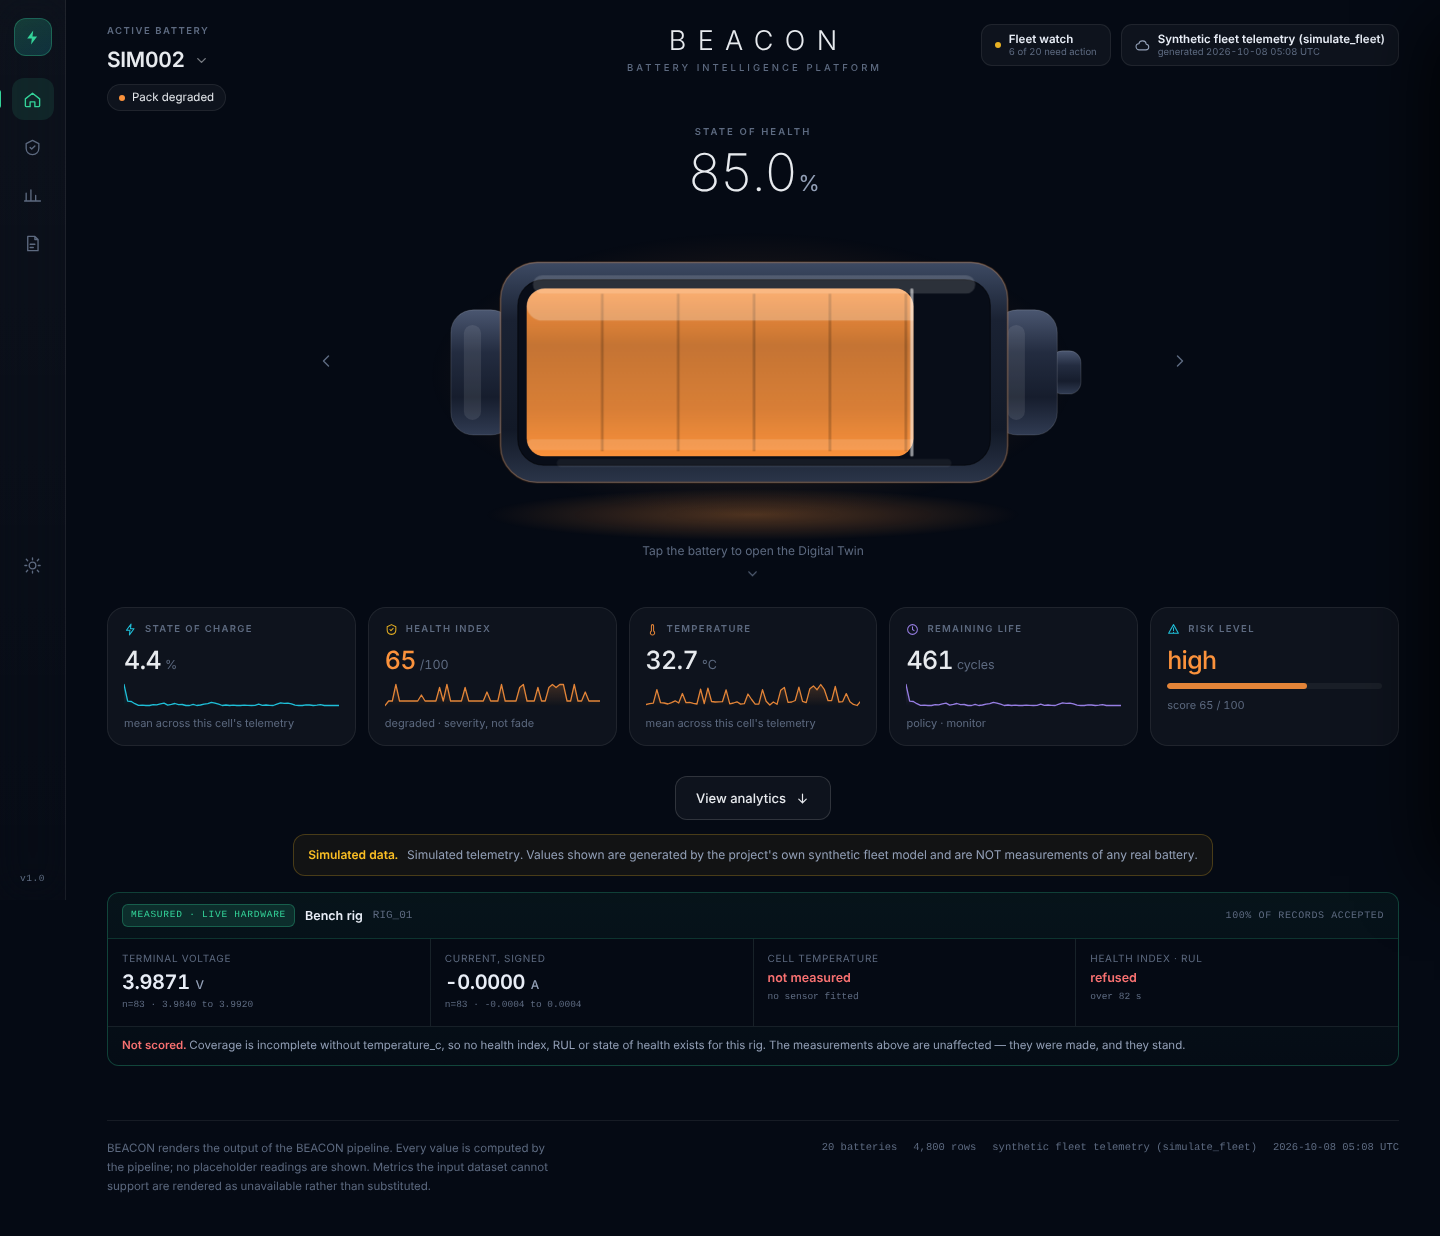
\includegraphics[width=\linewidth,height=0.5\textheight,keepaspectratio]{images/ui_overview.png}
    \caption{Overview screen of the BEACON dashboard on a synthetic fleet. The banner marks the values as simulated, and the panel at the bottom shows the measured bench-rig readings, with the health index and remaining life refused because no temperature channel exists.}
    \label{fig:uioverview}
\end{figure}

\begin{figure}[htbp]
    \centering
    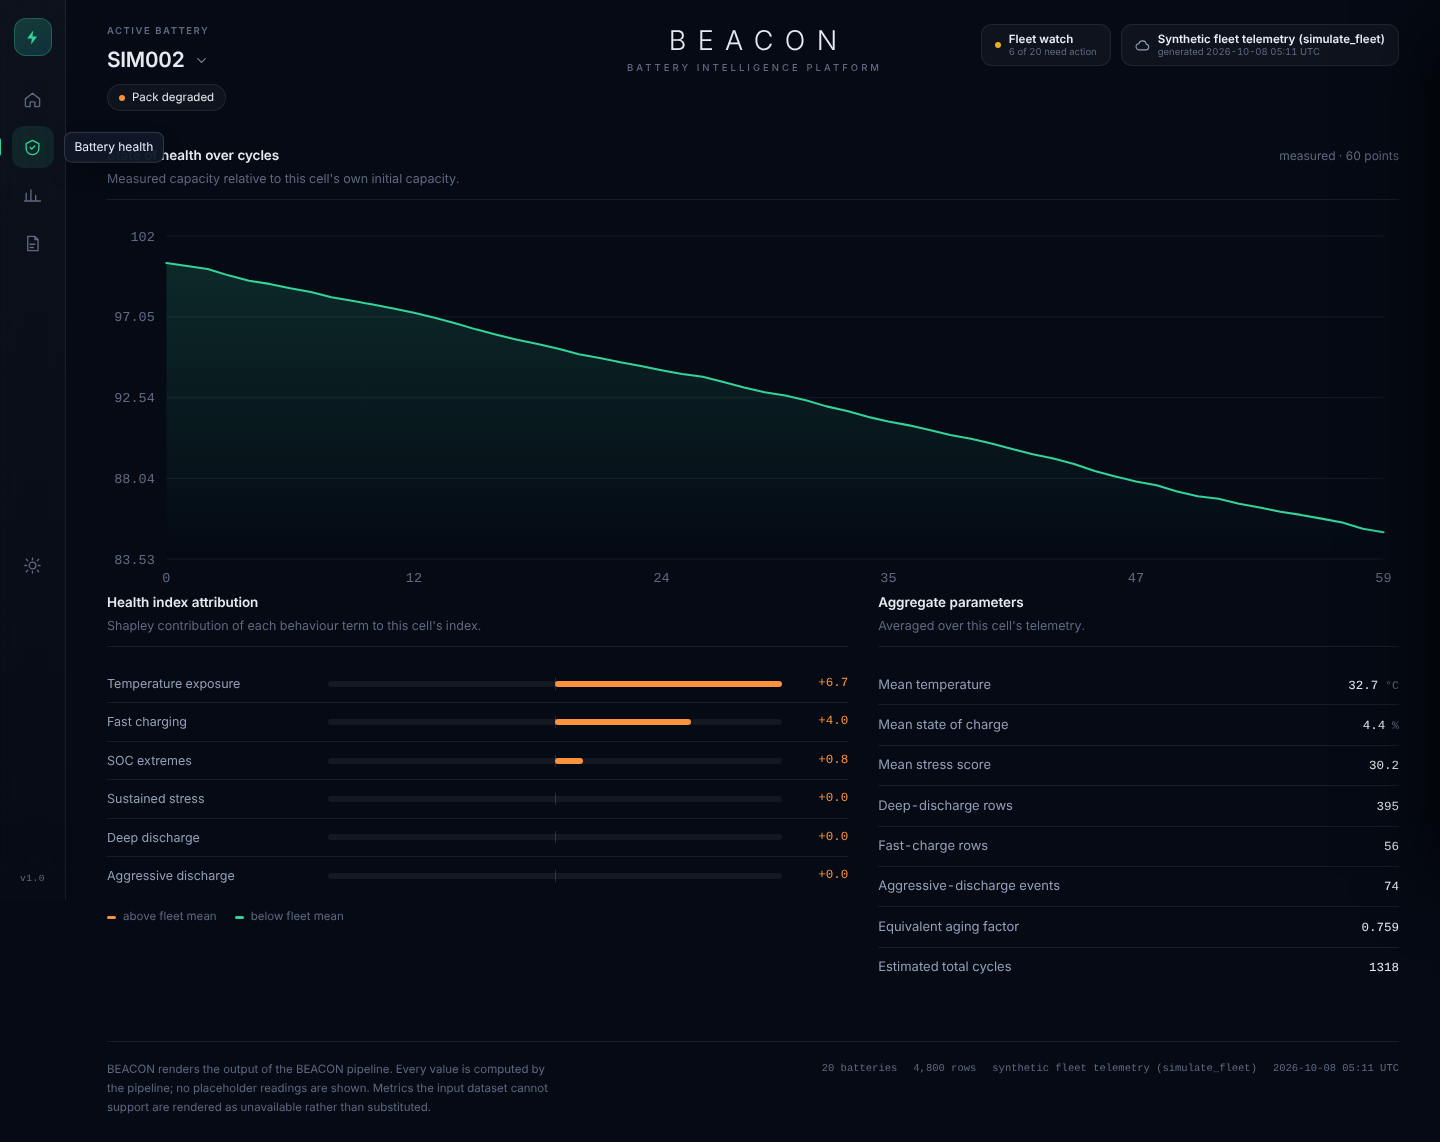
\includegraphics[width=\linewidth,height=0.5\textheight,keepaspectratio]{images/ui_health.png}
    \caption{Battery health screen: state of health over cycles for one battery, the attribution of its health index to behaviour terms, and its aggregate usage parameters (synthetic fleet).}
    \label{fig:uihealth}
\end{figure}

There are two deliberate absences. There is no database: the fleet store is in memory, and adding a database to the compose file would imply a persistence layer that does not exist, so the compose file says so. Persistence is the next substantial piece of work.

\section{HEALTH REPORT CARD}
\label{sec:impl-card}

The health report script renders the outputs as a plain-language card for one battery, in five parts: how healthy it is, how long it has left, what the usage is doing to it, what to do, and what the report cannot tell. Every figure carries its validation error band, which is taken from a file of measured bands and pinned by a test, and each output is labelled measured, estimate or heuristic. When ground truth exists, the card is followed by a check against the laboratory, which the card itself was not shown. Section~\ref{sec:res-card} reports a worked example.

\section{TESTING, CONTINUOUS INTEGRATION AND REPRODUCIBILITY}
\label{sec:impl-test}

There are 44 test modules, and three kinds of test are not the usual kind.

\begin{itemize}
    \item \textbf{Prose-to-evidence pinning.} A test ties every figure quoted in the documentation to the artifact that produced it, so re-running an experiment and forgetting to update a paragraph fails the build. It caught a stale figure that had already been published.
    \item \textbf{Cross-artifact structural tests.} The firmware's declared field set is compared as a set against the schema, and the documented schema table must equal the rendered one. Substring assertions had already let a defect through: a renamed field left the schema id untouched, so the sketch kept announcing a version it no longer spoke.
    \item \textbf{Known-defect pins.} Some tests assert behaviour that is not desirable, with a comment saying so, for example that the risk score is too coarse to see a sevenfold change in average stress. Changing it would silently re-score every published figure, so it is pinned and a future change has to be deliberate.
\end{itemize}

Continuous integration runs eight jobs: lint and type checking, the test suite on Python 3.10 and 3.12, a job that uninstalls the optional CAN dependency and re-runs the suite, a job that reproduces the headline benchmark end to end, a firmware compile for three targets, the gateway tests, the client build, and the Docker build. The job without the optional dependency exists because ``it is optional'' is otherwise an untested claim. The Python-version matrix exists because testing only the newest version lets a declared floor rot silently.

\section{CONTAINERISATION AND DEPLOYMENT}
\label{sec:impl-deploy}

The Docker image is multi-stage on a slim Python 3.12 base, with the compiler confined to the build stage, a non-root user, and a health check that polls service liveness. Docker Compose brings up the API, the gateway and the client, with the gateway held until the API reports healthy, and a separate study service writes the result CSVs back to the host. The system runs on a fresh clone with no hardware, no database, no API keys and no dataset download:

\begin{verbatim}
python main.py                     # end-to-end run
python scripts/run_serial_demo.py  # emulated rig
python -m pytest tests/ -q         # the test suite
docker compose up                  # API, gateway, client
\end{verbatim}

\section{CHAPTER SUMMARY}

This chapter described the realisation of the design: a shared scoring path fed by three transports through a narrow seam, a self-synchronising wire protocol with refusal gates at both record and capture level, a physical rig brought up in two stages, a three-service stack served from containers, and a test and CI strategy aimed at keeping the documentation and the code honest. What this implementation \emph{achieved} is reported in the next chapter.

%%%%%%%%%%%%%%%% ch5_results %%%%%%%%%%%%%%%%
\chapter{RESULTS AND DISCUSSION}
\label{ch:results}

This chapter reports what the system measured and interprets each result where it appears. Every number is traced to a committed artifact (Appendix~A). Errors are mean absolute errors in SOH (0.01 equals one percentage point) per cell, summarised as a median over cells with a 95\% bootstrap interval that resamples cells, unless stated otherwise. Results that failed are reported alongside those that worked.

\section{FITTED MODELS DO NOT SURVIVE A CHANGE OF PROTOCOL}
\label{sec:res-bench}

On the NASA benchmark (31 cells, nine cohorts; the isotonic signal ceiling for the target SOH is 0.569), every one of twelve published methods lost skill from leave-one-cell-out (LOBO) to leave-one-cohort-out (LOCO) validation (Table~\ref{tab:bench}). LOBO rank carried almost no information about LOCO rank (Spearman $\rho = +0.084$, $p = 0.795$, $n = 12$). Across fourteen scored methods, the spread of LOCO point estimates (2.06 in $R^2$) was smaller than the width of the best method's own interval (3.66).

\begin{table}[htbp]
	\caption{Benchmark on 31 NASA Cells in Nine Cohorts (Six of the Methods Shown); LOCO Intervals Are 95\% Bootstrap Over Folds}
	\centering
	\small
	\renewcommand{\arraystretch}{1.15}
	\setlength{\tabcolsep}{4pt}
	\begin{tabular}{|L{0.28\linewidth}|C{0.1\linewidth}|C{0.1\linewidth}|C{0.19\linewidth}|C{0.12\linewidth}|}
		\hline
		\textbf{Method} & \textbf{LOBO $R^2$} & \textbf{LOCO $R^2$} & \textbf{LOCO 95\% CI} & \textbf{LOCO MAE} \\
		\hline
		XGBoost & 0.732 & 0.459 & [$-2.80$, 0.86] & 7.62\% \\
		\hline
		Age-linear baseline & 0.483 & 0.406 & [$-0.43$, 0.51] & 10.71\% \\
		\hline
		ElasticNet & 0.609 & 0.355 & [$-1.65$, 0.76] & 10.31\% \\
		\hline
		GPR (Mat\'ern) & 0.725 & 0.207 & [$-3.72$, 0.43] & 17.06\% \\
		\hline
		Random forest & 0.773 & 0.150 & [$-1.09$, 0.90] & 10.67\% \\
		\hline
		LSTM (10-cycle windows) & 0.593 & $-0.185$ & [$-2.09$, 0.66] & 17.36\% \\
		\hline
	\end{tabular}
	\label{tab:bench}
\end{table}

Fig.~\ref{fig:benchbar} shows the same comparison for all fourteen scored methods: nearly every bar drops from the blue (LOBO) to the red (LOCO) value when the held-out unit changes from a cell to a whole protocol cohort.

\begin{figure}[htbp]
    \centering
    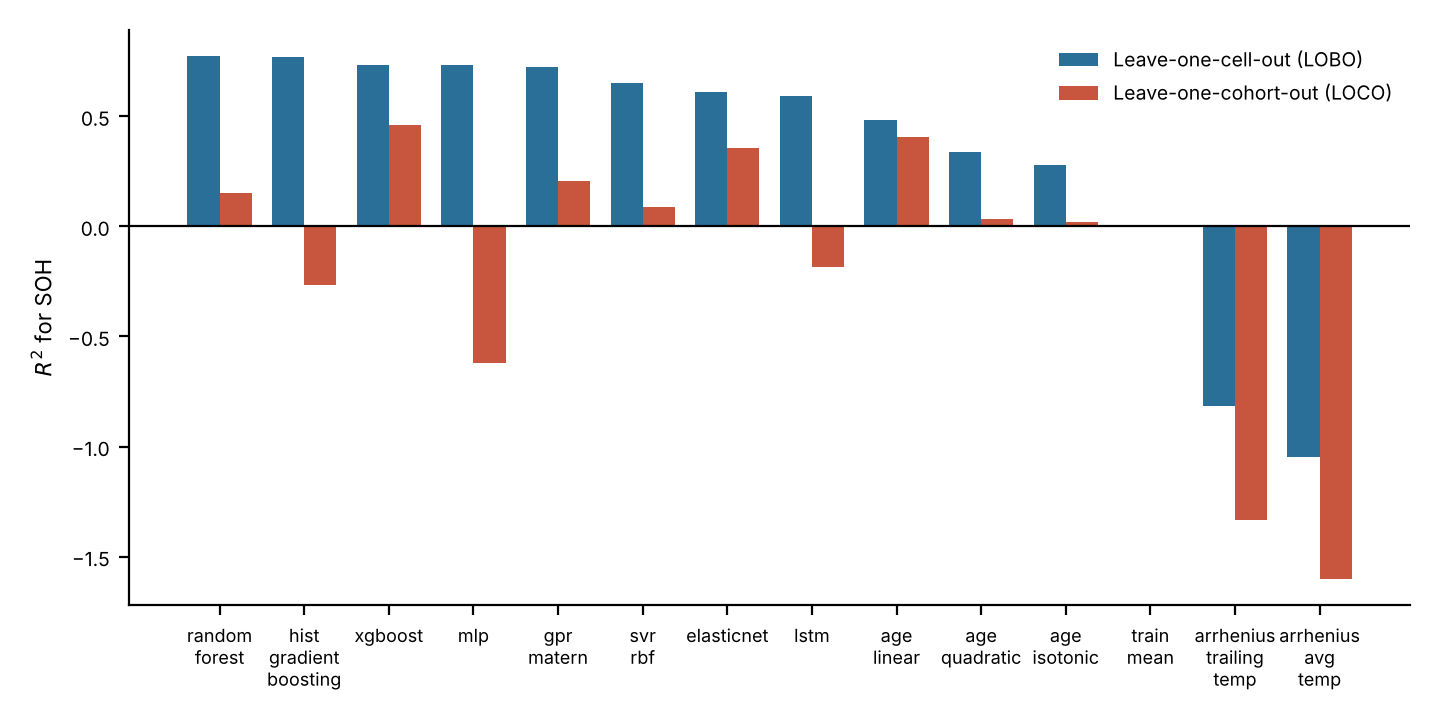
\includegraphics[width=\linewidth,height=0.35\textheight,keepaspectratio]{images/bench_lobo_loco.png}
    \caption{LOBO and LOCO $R^2$ for SOH for every scored method on the 31-cell NASA benchmark (data: \texttt{benchmark\_results.csv}). Skill measured across cells does not carry over to a new protocol.}
    \label{fig:benchbar}
\end{figure}


An ablation isolates where the skill comes from (Table~\ref{tab:ablation}). XGBoost on cycle number alone scored a LOCO $R^2$ of $-0.27$, and on behaviour features alone $-0.29$. Only their combination reached 0.459, while a straight line on cycle number reached 0.406. Shuffling each cell's capacity in time placed every LOCO interval at or below zero, so the harness does not manufacture skill. Usage features therefore added about 0.05 in $R^2$ over counting cycles, within the intervals.

\begin{table}[htbp]
	\caption{Feature Ablation and Shuffle Control (NASA SOH, LOCO)}
	\centering
	\small
	\renewcommand{\arraystretch}{1.15}
	\setlength{\tabcolsep}{4pt}
	\begin{tabular}{|L{0.38\linewidth}|L{0.17\linewidth}|C{0.12\linewidth}|C{0.2\linewidth}|}
		\hline
		\textbf{Run} & \textbf{Method} & \textbf{LOCO $R^2$} & \textbf{95\% CI} \\
		\hline
		All features (published) & XGBoost & 0.459 & [$-2.80$, 0.86] \\
		\hline
		All features (published) & Age-linear & 0.406 & [$-0.43$, 0.51] \\
		\hline
		Cycle number only & XGBoost & $-0.266$ & [$-1.15$, 0.82] \\
		\hline
		Behaviour features only & XGBoost & $-0.293$ & [$-0.72$, 0.80] \\
		\hline
		Shuffled in time (control) & Age-linear & $-0.039$ & [$-0.35$, $-0.004$] \\
		\hline
		Shuffled in time (control) & XGBoost & $-0.436$ & [$-1.44$, $-0.008$] \\
		\hline
	\end{tabular}
	\label{tab:ablation}
\end{table}

Temperature was the only usage factor with a consistent, correctly signed within-protocol relationship to fade (seven of seven cells), and its magnitude did not transfer between protocols. The rule-based risk score did not track measured fade either ($\rho = -0.27$, $p = 0.12$ on 33 cells), so it is labelled a heuristic.

\textbf{Interpretation.} No fitted method retains reliable skill under a change of protocol, and no method can be distinguished from another. This is the result that motivates the rest of the project: the estimators that ship fit nothing across cells.

\section{FIELD SOH FROM VOLTAGE, CURRENT AND TIME}
\label{sec:res-field}

Table~\ref{tab:field} compares three ohmic treatments at the primary window on 22 CALCE cells. The field correction matched the laboratory correction within its interval and measured five more cells than no correction. Sensitivity windows gave 1.2\% (4.05--3.55~V, 16 cells) and 1.9\% (3.85--3.55~V, 17 cells).

\begin{table}[htbp]
	\caption{Field SOH at the 3.90--3.60~V Window; Median Per-Cell Absolute Error Against Cycler Capacity, 95\% Bootstrap Interval Over Cells}
	\centering
	\small
	\renewcommand{\arraystretch}{1.15}
	\setlength{\tabcolsep}{4pt}
	\begin{tabular}{|L{0.38\linewidth}|C{0.1\linewidth}|C{0.11\linewidth}|C{0.15\linewidth}|C{0.1\linewidth}|}
		\hline
		\textbf{Ohmic correction} & \textbf{Cells} & \textbf{Median} & \textbf{95\% CI} & \textbf{Worst} \\
		\hline
		None & 12/22 & 4.3\% & 2.5--5.4\% & 6.4\% \\
		\hline
		Cycler resistance (laboratory only) & 12/20 & 1.4\% & 1.2--2.5\% & 5.6\% \\
		\hline
		\textbf{Step resistance (field)} & \textbf{17/21} & \textbf{1.7\%} & \textbf{1.4--4.3\%} & \textbf{10.3\%} \\
		\hline
	\end{tabular}
	\label{tab:field}
\end{table}

The denominators differ because a correction can only be scored on cells for which it exists: one cell never rests before discharging, so no step resistance exists for it, which gives 17 of 21 cells for the field arm and 17 of 22 once that cell is counted as refused. The three worst cells (6.4--10.3\%) are all Type~3, whose discharge switches rate within a cycle. Every refusal carries a stated cause: four storage and partial-protocol cells delivered 80--155 equivalent full cycles before any constant-current discharge crossed the window, so the reference gate refused them, and one cell never rests before discharging. Fig.~\ref{fig:track} tracks the estimate against every laboratory capacity test, and Fig.~\ref{fig:cells} shows every measured cell.

\begin{figure}[htbp]
    \centering
    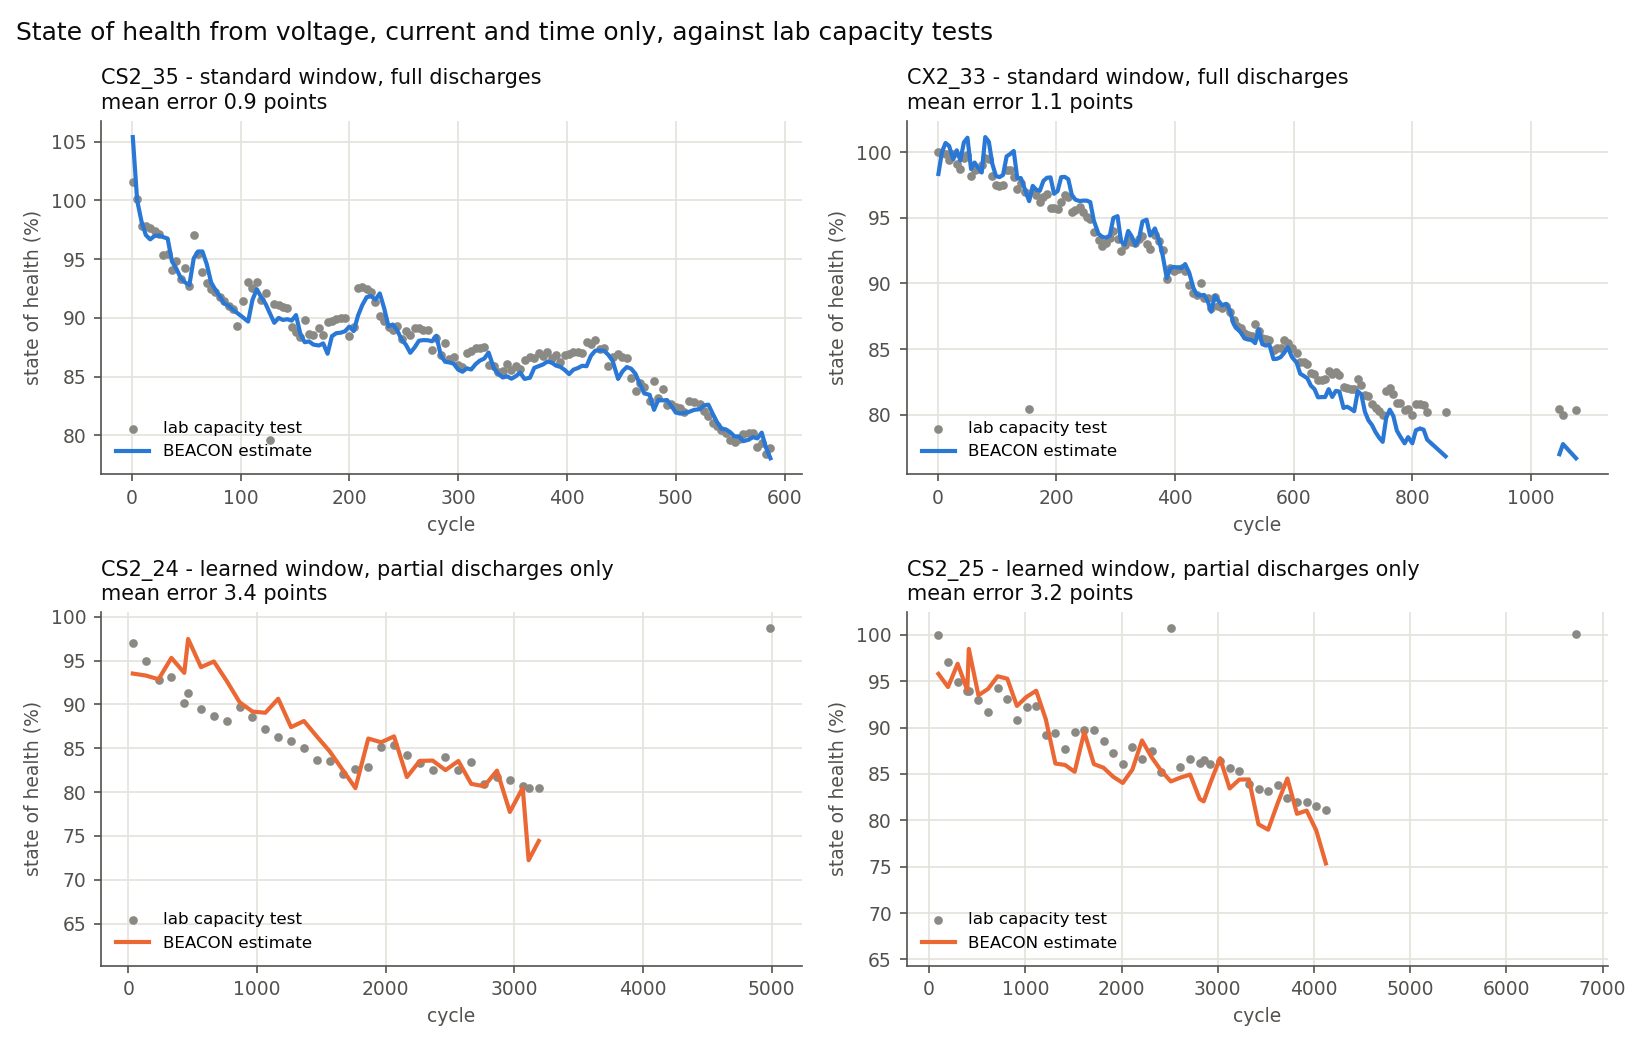
\includegraphics[width=\linewidth]{images/results_soh_tracking.png}
    \caption{SOH from voltage, current and time against every laboratory capacity test. Top: two constant-current cells, fixed window (mean error 0.9 and 1.1 points). Bottom: two cells of real partial cycling, learned window, estimate from partial discharges only (3.4 and 3.2 points).}
    \label{fig:track}
\end{figure}

\begin{figure}[htbp]
    \centering
    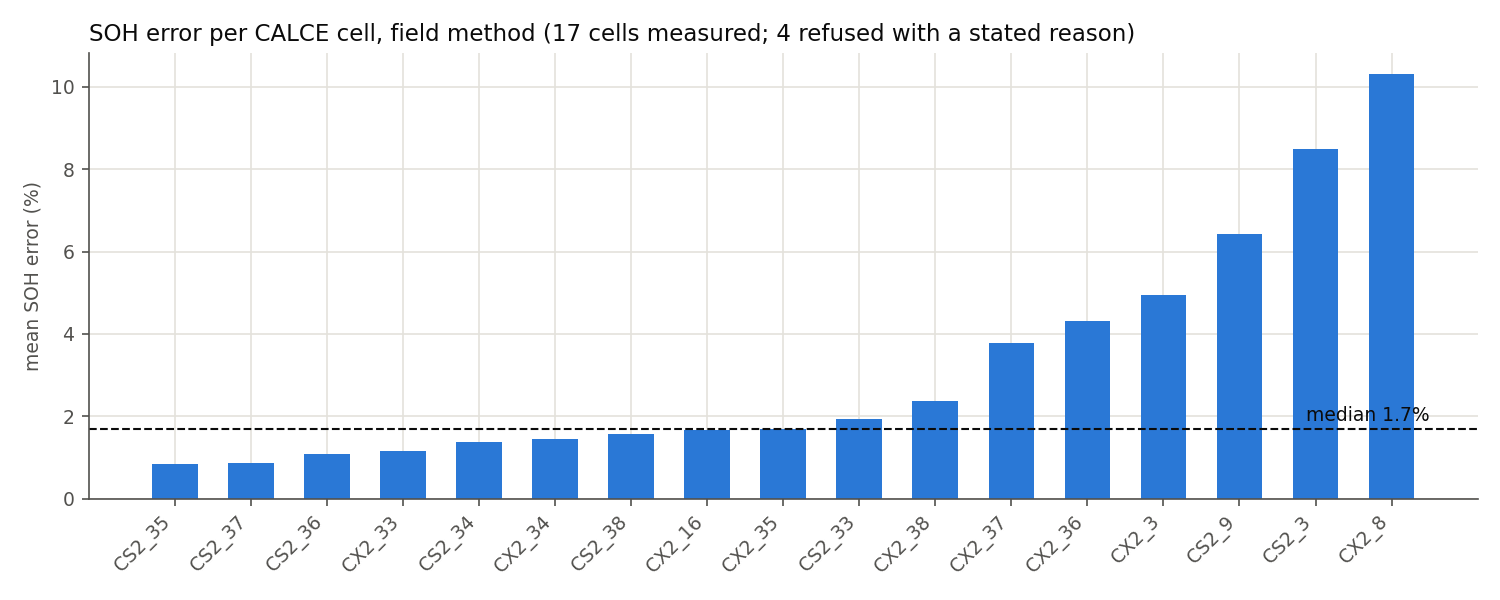
\includegraphics[width=\linewidth]{images/results_soh_per_cell.png}
    \caption{Mean absolute SOH error for every measured CALCE cell, field method; the dashed line is the median (1.7\%).}
    \label{fig:cells}
\end{figure}

\textbf{Interpretation.} Identifying resistance from the load step took the median error from 4.3\% to 1.7\% and the coverage from 12 to 17 cells, without any quantity the cycler computed. Two earlier figures were corrected downward by this work: an earlier 3.3\% SOH figure and an 88\% RUL figure had been scored against a reference capacity taken from each cell's whole life, which uses the future and which no BMS can hold.

\section{PARTIAL DISCHARGES}
\label{sec:res-partial}

On the four cells of real partial cycling (Table~\ref{tab:partial}), estimates use only the partial discharges preceding each laboratory check. Before the knee gate existed, the two near-empty cells were reported at 6.8\% and 12.8\% error while appearing confident. Learned windows on the 18 full-discharge cells have steepness 0.44--0.88, so any threshold between about 0.9 and 8 gives the same verdict on every cell and the chosen 2.0 is not tuned. As a control, the learned mode on those 18 cells measured 16 at a median of 1.95\%, beside 1.7\% for the fixed window, so it is a fallback and not a replacement.

\begin{table}[htbp]
	\caption{SOH from Real Partial Cycling (CALCE CS2 Types 5 and 6)}
	\centering
	\small
	\renewcommand{\arraystretch}{1.15}
	\setlength{\tabcolsep}{4pt}
	\begin{tabular}{|L{0.13\linewidth}|L{0.22\linewidth}|C{0.2\linewidth}|C{0.12\linewidth}|L{0.17\linewidth}|}
		\hline
		\textbf{Cell} & \textbf{Band} & \textbf{Learned window} & \textbf{Steepness} & \textbf{Result} \\
		\hline
		CS2\_24 & top of charge & 4.00--3.82~V & 0.83 & 3.4\% error \\
		\hline
		CS2\_25 & top of charge & 4.03--3.83~V & 0.82 & 3.2\% error \\
		\hline
		CS2\_5 & near empty & -- & 10.4 & refused (knee) \\
		\hline
		CS2\_6 & near empty & -- & 8.2 & refused (knee) \\
		\hline
	\end{tabular}
	\label{tab:partial}
\end{table}

\textbf{Interpretation.} The refusal is physics and not a tuned cut. On the plateau, window charge tracks capacity, while on the knee voltage is set by resistance and diffusion, so it measures how hard the cell is working instead. The scope is two cells per band, which shows the mechanism and is too few to quote a population error.

\section{RESISTANCE TRACKS THE INSTRUMENT}
\label{sec:res-r}

Against the cycler's internal-resistance column over each cell's life (20 cells carrying both values), the step resistance achieved a median Spearman correlation of 0.86, growth in the same direction on 19 of 20 cells, and a median growth of 1.26 times against the cycler's 1.29 times. This includes the partial-cycling cells (0.90 and 0.98), and the exception is a Type~3 cell. The levels differ, since the step value includes early polarisation, but the trends agree, which is what a power-fade indicator requires.

\section{REMAINING USEFUL LIFE}
\label{sec:res-rul}

At threshold 0.90, referenced to each cell's first cycles (17 cells), Table~\ref{tab:rul} reports accuracy by the true distance to end of life and by the prediction a user sees. Near end of life the estimate is a safe lower bound: it warns early and almost never late. Errors are predominantly early because these cells fade quickly at first and then more slowly, so a full-history line is steeper than the remaining fade.

\begin{table}[htbp]
	\caption{RUL to 90\% Capacity. Left: By True Cycles to End of Life. Right: By Predicted Cycles, With the 90\% Range of (True $-$ Predicted)}
	\centering
	\footnotesize
	\renewcommand{\arraystretch}{1.15}
	\setlength{\tabcolsep}{3pt}
	\begin{tabular}{|C{0.1\linewidth}|C{0.11\linewidth}|C{0.1\linewidth}|C{0.11\linewidth}|C{0.14\linewidth}|C{0.15\linewidth}|}
		\hline
		\textbf{True} & \textbf{Within $\pm$20} & \textbf{Median err.} & \textbf{Predicted} & \textbf{Lasted $\ge$ pred.} & \textbf{90\% range} \\
		\hline
		0--25 & 73\% & 9.6 & 0--25 & 95\% & $+1$ to $+82$ \\
		\hline
		25--50 & 44\% & 22.8 & 25--50 & 88\% & $-14$ to $+129$ \\
		\hline
		50--100 & 15\% & 42.7 & 50--100 & 85\% & $-40$ to $+141$ \\
		\hline
		200--400 & 0\% & 144 & -- & -- & -- \\
		\hline
	\end{tabular}
	\label{tab:rul}
\end{table}

Scored against a reference capacity taken as the 95th percentile of the cell's whole record, the same estimator was within $\pm$20 cycles 88\% of the time near end of life. That reference uses the future, which no BMS can hold. Against the cell's own early capacity the figure is 73\%, and that is the figure reported. Fig.~\ref{fig:rul} summarises the result.

\begin{figure}[htbp]
    \centering
    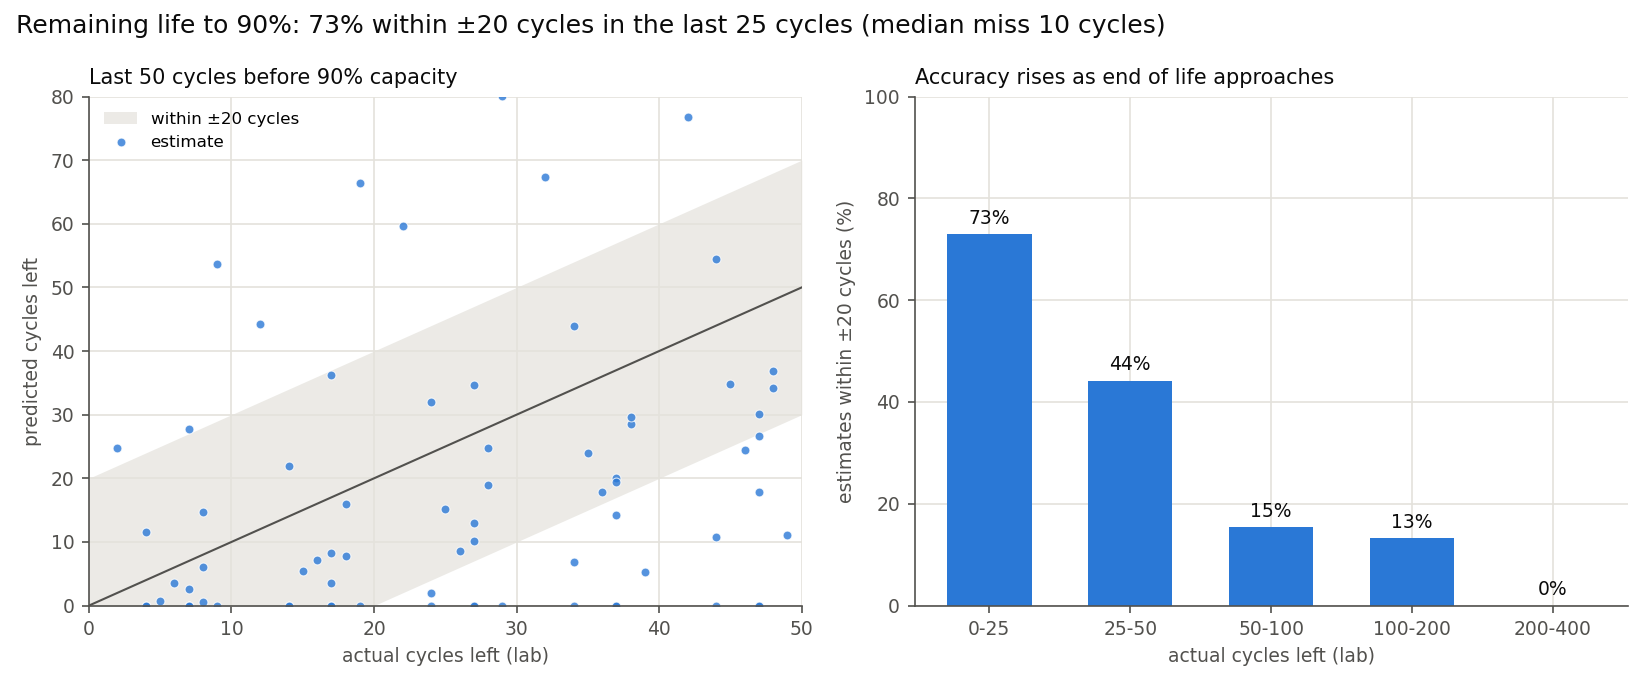
\includegraphics[width=\linewidth]{images/results_rul.png}
    \caption{RUL to 90\% capacity. Left: predicted against actual cycles left in the last 50 cycles. Right: share of estimates within $\pm$20 cycles by actual distance to end of life.}
    \label{fig:rul}
\end{figure}

\textbf{Interpretation.} The ``within $\pm$20 cycles'' claim is true near end of life and false far from it (0\% at 200 or more cycles out), so it is reported with its condition and not bare. The conservative direction is a property of the 90\% threshold on these cells and is not a general guarantee. At an 85\% threshold the median bias near end of life turns positive (+6.7 cycles within 25 cycles of end of life), so the estimate runs late there and only 62.8\% of estimates fall within $\pm$20 cycles. The conventional 80\% end-of-life threshold is not validated on CALCE, because its full-discharge trajectories end near 0.81 and only one cell of 22 crosses 0.80.

\section{RUL WHEN COMPLETE DISCHARGES ARE RARE}
\label{sec:res-sparse}

A driver who seldom fully discharges produces few complete discharges (CS2\_24 has 18 in 1,617). Four methods were evaluated on the same sparse evidence (Table~\ref{tab:sparse}). Sparsity is real on the partial-cycling cells and emulated as one complete discharge in 50 on the constant-current cells.

\begin{table}[htbp]
	\caption{RUL from Sparse Complete Discharges; None Is Accurate Enough to Report}
	\centering
	\small
	\renewcommand{\arraystretch}{1.15}
	\setlength{\tabcolsep}{4pt}
	\begin{tabular}{|L{0.4\linewidth}|L{0.46\linewidth}|}
		\hline
		\textbf{Method} & \textbf{Outcome} \\
		\hline
		Sparse capacity, standard minimum & Refuses every point (never reaches 30) \\
		\hline
		Field SOH trajectory & Answers 62\%; median miss 79 cycles when predicting under 25 \\
		\hline
		Field SOH scaled by the cell's own complete discharges & Over-corrects; errors turn late near end of life \\
		\hline
		Sparse capacity, minimum lowered to 5 (post hoc) & 0\% within $\pm$20 cycles; misses late \\
		\hline
	\end{tabular}
	\label{tab:sparse}
\end{table}

The failure of the field-trajectory method has a clean cause. Near 0.90, field SOH reads a median 1.1 points below capacity (measured in a first pass of this study, not kept as a separate artifact). Because fade near the threshold is slow, that small bias moves the 0.90 crossing a median 56 cycles early. An SOH error that is acceptable as a health figure thus becomes large as a time to threshold. None of the four is reported, and the system refuses RUL for partial-only records and states that this was tested.

\section{WHEN THE EVIDENCE SUFFICES}
\label{sec:res-suff}

Three questions were fixed before the study and scored at every laboratory check on 19 cells. First, \emph{count does not predict accuracy}: median error was 0.75\% at 6--10 usable readings and 1.97\% beyond 60, because error grows with age as the approximation in Eq.~\eqref{eq:soh} drifts. A rule of high confidence after a fixed number of discharges therefore has no support. Second, \emph{consistency does} (Table~\ref{tab:suff}). The pooled Spearman correlation between $u$ and absolute error was 0.48. Within cells it was weaker (median 0.14, positive in 14 of 19), so $u$ chiefly separates unreliable cells and periods and does not rank readings within a good one.

\begin{table}[htbp]
	\caption{Error by the Consistency Criterion of Eq.~\eqref{eq:u}}
	\centering
	\small
	\renewcommand{\arraystretch}{1.15}
	\setlength{\tabcolsep}{4pt}
	\begin{tabular}{|L{0.34\linewidth}|C{0.12\linewidth}|C{0.1\linewidth}|C{0.13\linewidth}|C{0.14\linewidth}|}
		\hline
		\textbf{Readings} & \textbf{Points} & \textbf{Cells} & \textbf{Median error} & \textbf{90th percentile} \\
		\hline
		$u \le 0.01$ (consistent) & 8,993 & 16 & 1.3\% & 4.4\% \\
		\hline
		$u > 0.01$ (inconsistent) & 2,168 & 13 & 5.1\% & 21.9\% \\
		\hline
	\end{tabular}
	\label{tab:suff}
\end{table}

Third, \emph{reference size}: in the study's own scoring, larger references reduced error (one discharge 3.6\%, five 2.0\%, ten 1.3\%), but on the field-study metric ten versus five changed the median only from 1.681\% to 1.665\%, so the estimator retains five.

\section{EXTERNAL VALIDATION ON A SECOND DATASET}
\label{sec:res-oxford}

The estimator was applied to the eight Oxford cells without re-tuning. Arms, reference and scoring were fixed before the run. The reference is each cell's first characterisation, and truth is 1C capacity relative to it. Because each characterisation block begins under load, no rest-to-load step exists, so the 1C window is uncorrected.

\begin{table}[htbp]
	\caption{External Validation on Eight Oxford Cells: Median and Worst Per-Cell Mean Absolute SOH Error}
	\centering
	\small
	\renewcommand{\arraystretch}{1.15}
	\setlength{\tabcolsep}{4pt}
	\begin{tabular}{|L{0.5\linewidth}|C{0.1\linewidth}|C{0.12\linewidth}|C{0.1\linewidth}|}
		\hline
		\textbf{Window} & \textbf{Cells} & \textbf{Median} & \textbf{Worst} \\
		\hline
		Fixed 3.90--3.60~V, 1C discharge & 8/8 & 3.0\% & 4.0\% \\
		\hline
		Fixed 3.90--3.60~V, C/18 pseudo-OCV & 8/8 & 3.2\% & 3.4\% \\
		\hline
		Learned window, 1C discharge & 8/8 & 2.3\% & 3.6\% \\
		\hline
	\end{tabular}
	\label{tab:oxford}
\end{table}

All eight cells were measured (Table~\ref{tab:oxford}). The near-equilibrium C/18 window was not more accurate than the 1C window, so on this blend cathode the residual error stems from the curve changing shape with age and not from ohmic sag, consistent with the stated approximation of Eq.~\eqref{eq:soh}.

\paragraph{A real drive-cycle discharge.} The drive-cycle discharge of Cell~1 has current between $-5.0$ and $+1.6$~A. Resistance from its own 1,575 current steps of at least 0.2~A gave a median of 21~m$\Omega$ (interquartile 19--24). The discharge is itself partial (it stops at about 65\% depth), so a coverage window (4.08--3.78~V) was chosen from the corrected curve's span alone, before any comparison was computed. In it the drive-cycle reading, corrected per sample and fitted monotonically, was 0.2625~Ah, against 0.2661~Ah from the same cell's 1C constant-current discharge, a difference of 1.4\%. Both lay about 13\% below the C/18 reading in that window, so the rate effect cancels in a ratio of like with like but would bias one that mixed rates. This is a single discharge and demonstrates the mechanism, not a population error.

\paragraph{Remaining life at 80\%.} The Oxford trajectories cross the 80\% convention, so the shipped RUL estimator was scored there unchanged. When it predicted fewer than 500 cycles to 80\%, the cell lasted at least that long in 97\% of cases (36 estimates, 5 cells). Precision is low: the median miss is 385 cycles against characterisations 100 cycles apart. The guarantee also weakens with distance, since predictions of 500 to 1,000 cycles were met or exceeded only 80\% of the time (25 estimates, 5 cells).

\section{A THIRD DATASET AND KNOWING WHEN TO REFUSE}
\label{sec:res-xds}

The NASA files (18650 cells, ambient 4--44~$^\circ$C) were read from their original MATLAB form and scored the same way, unchanged. The estimator was poor on NASA overall, with a median per-cell error of 9.2\% over 27 cells, and it depended on temperature: 1.7\% in the 43~$^\circ$C cohort and 12--14\% at 4 and 22~$^\circ$C. The step resistance captures only the ohmic part of the overpotential, and at low temperature the charge-transfer and diffusion parts, which grow with age, move the curve through the window.

The consistency uncertainty, with its tolerance fixed on CALCE, was applied unchanged. On NASA, estimates it labelled HIGH or MEDIUM had a median per-cell error of 4.5\%, while those labelled LOW had 13.2\% (within three SOH points: 49\% versus 12\%). The failure on unseen conditions was thus largely signalled by the estimator itself.

For contrast, a gradient-boosted model on three window features, the setting where fitting looks best, reached 0.7\% under leave-one-cell-out within Oxford and 1.2\% within CALCE, but 6.7\% when moved from Oxford to NASA and 5.5\% from CALCE to Oxford. Validation inside one dataset overstated transferable accuracy four- to tenfold.

\section{SYSTEM AND HARDWARE RESULTS}
\label{sec:res-system}

\subsection{Bench Rig Captures}

Three captures are committed (Table~\ref{tab:captures}). The first is a counter-example: a board with no sensors attached, whose synthetic profile still scores, and which is kept and labelled as such.

\begin{table}[htbp]
	\caption{Bench Rig Captures}
	\centering
	\footnotesize
	\renewcommand{\arraystretch}{1.15}
	\setlength{\tabcolsep}{3pt}
	\begin{tabular}{|L{0.22\linewidth}|L{0.2\linewidth}|C{0.12\linewidth}|L{0.22\linewidth}|}
		\hline
		\textbf{Capture} & \textbf{Declared channels} & \textbf{Records} & \textbf{Measured} \\
		\hline
		Stage A (no sensors) & all, from stubs & 151 & Synthetic, not a hardware result \\
		\hline
		Stage B voltage & $t$, $v$, $i$, SOC (INA219 up, LM35 refused) & 83 over 82~s & 3.9871~V (sd 1.9~mV); current at the $\pm$0.4~mA noise floor \\
		\hline
		Temperature demo & $t$, $t_c$ (LM35 up, INA219 refused) & 85 over 84~s & 32.11~$^\circ$C (sd 0.086~$^\circ$C) \\
		\hline
	\end{tabular}
	\label{tab:captures}
\end{table}

In both real captures the cadence held at 1.000~s with no gaps and a monotonic time base. Every measured voltage is an exact multiple of the INA219's 4~mV bus LSB, which is what a genuine read from that part looks like and what a fabricated one would not. The sensor-complement declaration worked as designed: the firmware named the sensor that failed at boot, declared only the channels it could supply, and the host scored those and refused the rest by name. The first real board also exposed a baud-rate fault (the CH340 bridge accepts only 9600 and 19200 baud), which the refusal wording named as a cause and which led to the fix.

Fig.~\ref{fig:rigcapture} plots the Stage B capture and Fig.~\ref{fig:uievidence} shows how the dashboard presents it.

\begin{figure}[htbp]
    \centering
    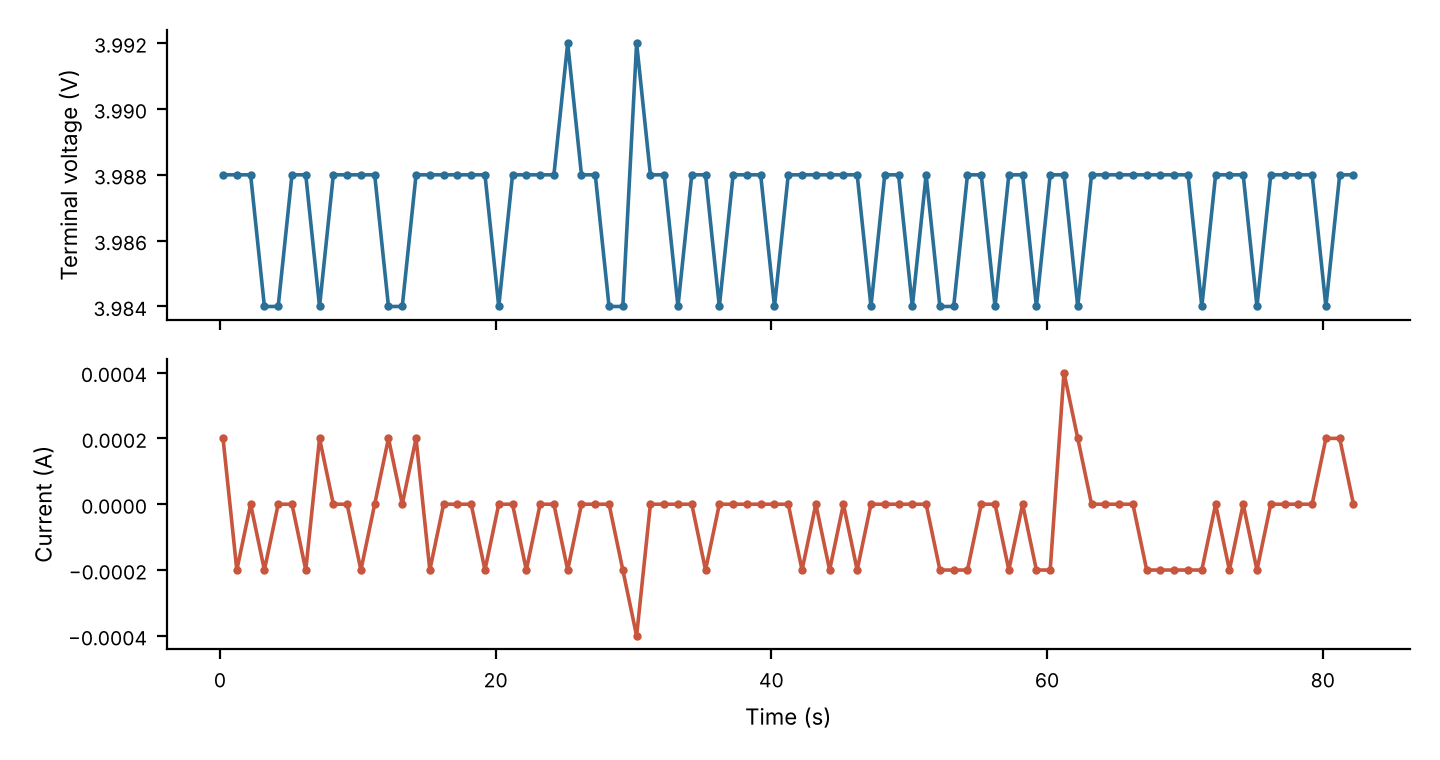
\includegraphics[width=\linewidth,height=0.35\textheight,keepaspectratio]{images/rig_capture.png}
    \caption{Stage B capture from the bench rig (83 frames over 82~s, one cell at rest). Voltage moves between 3.984 and 3.992~V in steps of the INA219's 4~mV LSB, and current stays at the $\pm$0.4~mA noise floor.}
    \label{fig:rigcapture}
\end{figure}

\begin{figure}[htbp]
    \centering
    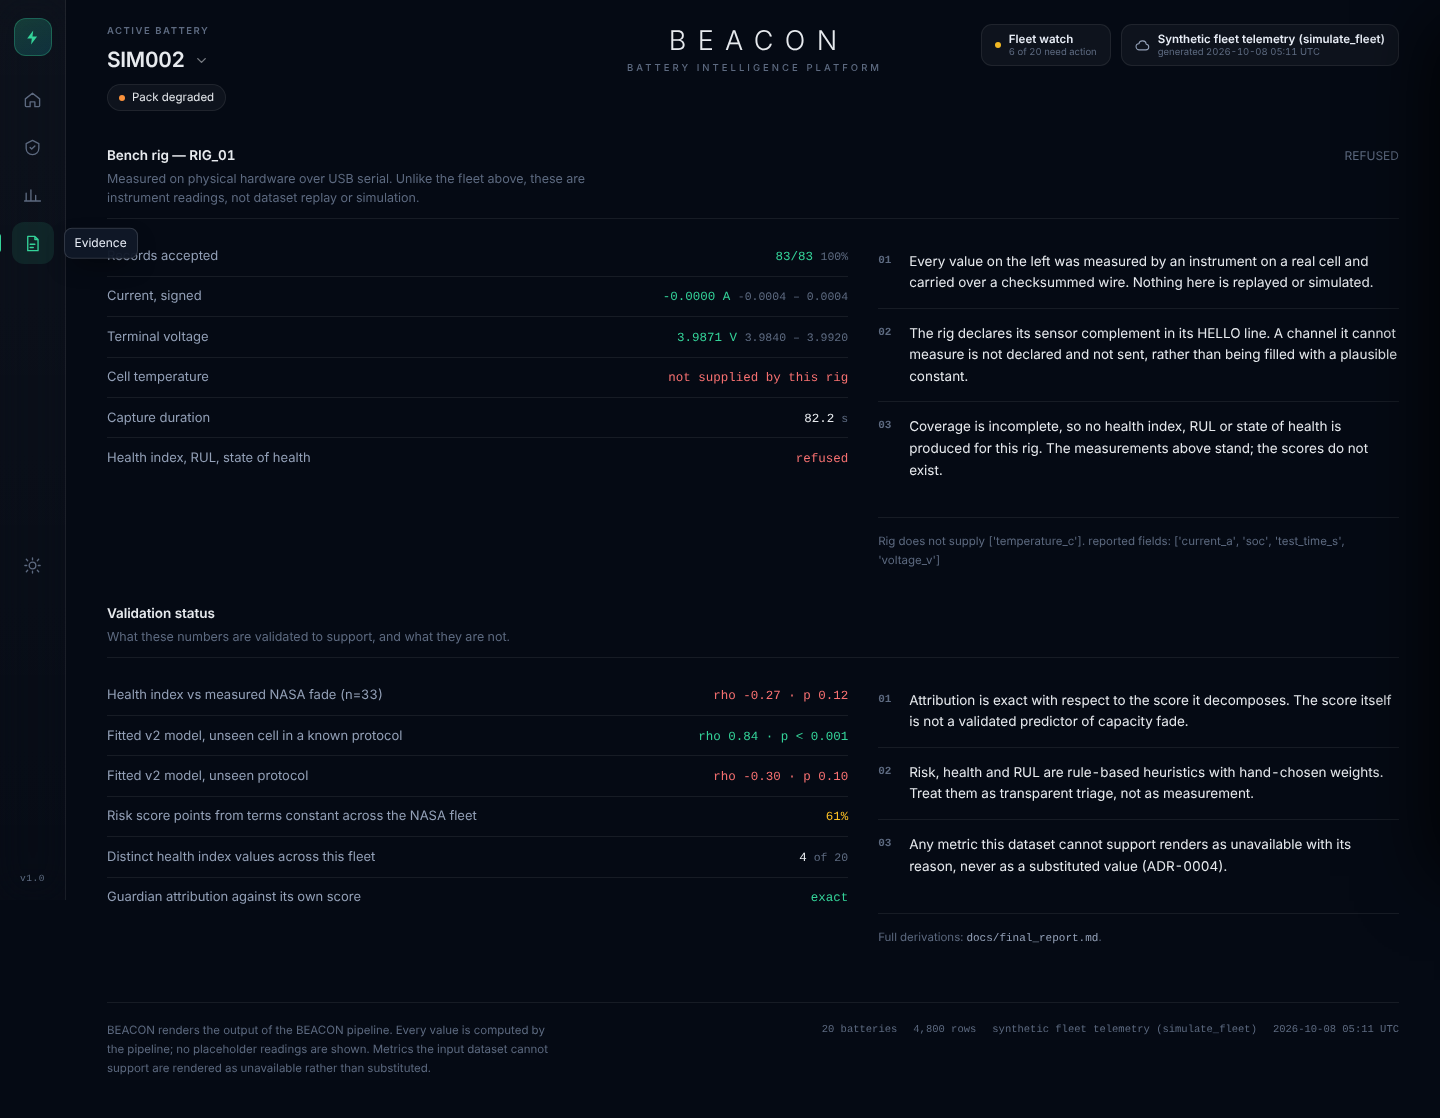
\includegraphics[width=\linewidth,height=0.45\textheight,keepaspectratio]{images/ui_evidence.png}
    \caption{Evidence view of the BEACON dashboard for the bench rig: 83 of 83 records accepted, voltage and current as measured, temperature reported as not supplied, and the health index, remaining life and state of health refused because coverage is incomplete.}
    \label{fig:uievidence}
\end{figure}


\subsection{Fault Injection}

Faults injected into a real capture behaved as designed: a corrupted byte failed its checksum, a NaN field was rejected, a reversed timestamp refused the capture, and a missing sensor was refused by name. The injection also exposed one defect, since corrected: a 999~V reading passed the field range, which is wide so that packs are admissible. Records outside 0--5~V are now rejected when the source declares a single cell.

\subsection{What the Hardware Result Does and Does Not Show}

The captures demonstrate that the transport, the protocol, the gate and the refusal path work against real silicon. They are one cell, at rest, for under 90~s, with no load step and no charge or discharge cycle. They are \emph{not} a validation of the health, RUL or risk models, which were fitted on cycled research cells and cannot be confirmed or refuted by a cell that was never cycled. Sensor accuracy against a reference meter was not measured, and no discharge has yet been recorded on the rig.

\section{A WORKED EXAMPLE: THE REPORT CARD}
\label{sec:res-card}

Fig.~\ref{fig:card} abridges the report card for CALCE cell CS2\_35 as it would have read at cycle 90. The pipeline saw voltage, current and time only.

\begin{figure}[htbp]
    \centering
    {\footnotesize
\begin{verbatim}
1. HOW HEALTHY IT IS
   91.0% state of health  [MEASURED]   State: WARNING
2. HOW LONG IT HAS LEFT
   About 5 cycles until it falls to 90% of its early
   capacity.  [ESTIMATE]
3. WHAT YOUR USAGE IS DOING TO IT
   No temperature was measured, so heat exposure cannot
   be assessed.
4. WHAT TO DO
   Capacity fade is measurable. Keep monitoring.
5. WHAT THIS REPORT CANNOT TELL YOU
   - Scoring skipped: required channels not supplied.

CHECK AGAINST THE LAB (the card was not shown this)
   Lab capacity at cycle 90: 91.4%; card said 91.0%
   Cell actually crossed 90% at cycle 146: 56 cycles
   after cycle 90; card said 5
\end{verbatim}}
    \caption{Abridged health report card for CS2\_35 at cycle 90, with the laboratory check.}
    \label{fig:card}
\end{figure}

The health figure is within half a point. The remaining-life figure is 51 cycles early, which is the conservative bias the RUL study measured at that distance (median $-32$ cycles at 50--100 cycles out), and it is the reason the card prints its own accuracy beside the number and not the number alone. Only temperature is offered as a usage finding, because it is the one behaviour-to-ageing link that survived testing, in direction only.

\section{DISCUSSION}
\label{sec:discussion}

\paragraph{Conditioning moved accuracy; model choice did not.} Across fourteen scored methods, LOCO differences were smaller than the uncertainty on any one of them. Three conditioning decisions, by contrast, changed error by multiples. Refusing truncated discharges took the worst cell from 52\% to about 10\%. Identifying resistance from the load step took the median from 4.3\% to 1.7\% and coverage from 12 to 17 cells. Refusing knee windows converted 6.8--12.8\% errors into refusals. For a BMS software layer, the leverage lies in what is measured and how it is conditioned, not in the regressor that follows. The first of these was a misdiagnosis corrected during the project: the 52\% worst case had been attributed to loss of active material, when it was actually truncated discharges being read as full ones.

\paragraph{Reference definitions change conclusions.} Two results moved when the reference was made one a BMS can hold: RUL accuracy fell from 88\% to 73\%, and a partial-discharge reference formed from a late discharge produced a large error until the timing gate existed. Validation should use the reference the deployed system will have.

\paragraph{Threshold crossings amplify small biases.} A 1.1-point SOH bias, unremarkable as a health figure, shifted predicted end of life by about 56 cycles. Any RUL built on an estimated rather than measured SOH inherits this, and should be evaluated as a time to threshold and not through SOH error.

\paragraph{Sufficiency is measurable.} Treating ``enough data'' as a count is intuitive and here wrong, because the estimator's error is dominated by age-related drift and not sampling. The consistency of readings is observable without ground truth and separates 1.3\% from 5.1\% median error, which gives a BMS layer a principled way to report ``not yet'' for a battery it has never seen.

\paragraph{Limitations.}
\begin{itemize}
    \item \emph{Temperature.} On NASA cells at 4 and 22~$^\circ$C the estimator erred by 12--14\%. The low-confidence label marked most of these readings, but a temperature-aware correction is future work.
    \item \emph{Two cathode families, single cells, one real drive cycle.} Packs add cell-to-cell imbalance, thermal gradients and balancing currents, and the flat plateau of lithium iron phosphate would challenge the window method directly.
    \item \emph{Two cells per partial-cycling band.}
    \item \emph{End of life:} validated at 90\% on CALCE, and at 80\% on Oxford only as a conservative bound with low precision.
    \item \emph{Apparent resistance} depends on the logger's sample interval and is comparable within a record, not across loggers.
    \item \emph{No hardware discharge} has yet been recorded on the bench rig, and the heuristic risk layer is not validated.
\end{itemize}

\section{VALIDATION SUMMARY}

Table~\ref{tab:summary} lists the outputs by status. Claims that failed or were never tested are listed, because that is what makes the others believable.

\begin{table}[htbp]
	\caption{Status of the Main Outputs}
	\centering
	\footnotesize
	\renewcommand{\arraystretch}{1.15}
	\setlength{\tabcolsep}{3pt}
	\begin{tabular}{|L{0.34\linewidth}|L{0.34\linewidth}|L{0.2\linewidth}|}
		\hline
		\textbf{Output} & \textbf{Result} & \textbf{Status} \\
		\hline
		Capacity health (full discharges) & 1.7\% median, 17 of 22 cells & Validated \\
		\hline
		Capacity health (partial discharges) & 3.2--3.4\%, 2 cells & Validated, 2 cells \\
		\hline
		Resistance health & Same direction on 19 of 20 cells & Validated \\
		\hline
		RUL near end of life & 73\% within $\pm$20 cycles & Validated, 90\% threshold \\
		\hline
		RUL far from end of life & 0\% at 200--400 cycles & Not valid (shown with band) \\
		\hline
		RUL from sparse complete discharges & Four methods, none accurate & Refused \\
		\hline
		Second dataset (Oxford) & 3.0\% median, 8 of 8 cells & Validated \\
		\hline
		Third dataset (NASA) & 9.2\% overall, 1.7\% at 43~$^\circ$C & Fails outside warm conditions \\
		\hline
		Fitted models across protocols & Best LOCO $R^2$ 0.459, CI [$-2.80$, 0.86] & Not generalising \\
		\hline
		Heuristic risk score & $\rho=-0.27$, $p=0.12$ & Labelled heuristic \\
		\hline
		Telemetry on hardware & 83/83 frames, 1.000~s cadence & Validated (acquisition only) \\
		\hline
		Health from a real rig discharge & No discharge recorded & Not tested \\
		\hline
		Packs, LFP, large-scale drive cycles & No data & Not tested \\
		\hline
	\end{tabular}
	\label{tab:summary}
\end{table}

%%%%%%%%%%%%%%%% ch6_conclusion %%%%%%%%%%%%%%%%
\chapter{CONCLUSION AND FUTURE WORK}
\label{ch:conclusion}

This project asked whether a software layer above a battery management system can turn voltage, current and time into a trustworthy battery health report, and when it should decline to answer. It built BEACON, a three-tier system that ingests telemetry from a CAN bus, a USB serial rig or research datasets, converges all three on one schema, and scores them through one shared pipeline that is served to a React dashboard.

The research answer is that such a layer can measure cell health without any model trained on other cells. On 22 CALCE cells it delivered capacity health at 1.7\% median error (95\% CI 1.4--4.3\%) on 17 cells, with every one of the five refusals explained, and a resistance trend that tracked the laboratory instrument in the same direction on 19 of 20 cells. Partial-discharge capacity health reached 3.2--3.4\% on two cells of real top-of-charge cycling, with a physical rule that refuses windows on the discharge knee. Unchanged, the estimator measured all eight cells of an independent NMC/LCO dataset at 40~$^\circ$C with a 3.0\% median error, and a real drive-cycle discharge read within 1.4\% of a constant-current one. Remaining useful life extrapolated from each cell's own fade was within $\pm$20 cycles 73\% of the time in the last 25 cycles before 90\% capacity, and at that threshold behaved as a safe lower bound.

Equally important are the results that failed. Twelve published fitted methods all lost skill when the held-out unit changed from a cell to a protocol cohort, and no ranking of methods was supportable, which is why the shipped estimators fit nothing across cells. RUL from sparse complete discharges was tested by four methods and refused. The estimator was poor on cold NASA cells (12--14\%), but its own consistency criterion, with a tolerance fixed on CALCE, marked those failures: 4.5\% median error when it said high or medium confidence against 13.2\% when it said low.

On the engineering side, the system refuses to output a number it cannot justify. Nine gates return a refusal as a value instead of an exception, the wire protocol is self-synchronising with record-level and capture-level checks, and 44 test modules and an eight-job CI pipeline pin the documentation to the artifacts that produced it. A physical rig built on a NodeMCU ESP8266 with an INA219 and an LM35 streamed 83 of 83 checksummed frames at a measured 1.000~s cadence. That validates data acquisition. It does not validate health estimation, because no discharge has yet been recorded on the rig.

Each output therefore carries a measured error band and is withheld when its evidence is missing or inconsistent, and the criterion that makes that decision was itself validated against laboratory truth.

\section{LIMITATIONS}

The scope is single cells: LCO for development, an NMC/LCO blend pouch for external validation, mostly at constant current, with one real drive-cycle discharge. Packs, lithium iron phosphate and temperature-dependent capacity correction are not covered. The conventional 80\% end-of-life threshold is not validated on CALCE, and the Oxford results at 80\% are a conservative bound with low precision. The heuristic risk layer is not validated against measured degradation. The bench rig has been run on one cell, at rest, for under 90~s, and its two sensors have not yet operated in the same capture.

\section{FUTURE WORK}

In order of dependency:

\begin{enumerate}
    \item \textbf{Hardware validation.} Capture a load step and a full constant-current discharge on the rig with all three channels real, compare the resulting capacity with an independent charger/discharger, and measure sensor accuracy against a reference meter. Then repeat on more than one cell.
    \item \textbf{Protocol hardening.} Replace the XOR checksum with a CRC-8 at the same cost, which detects burst errors and byte transpositions the XOR form cannot.
    \item \textbf{Removing the remaining silent default.} The serial path no longer assumes a rated capacity, but the CAN and batch paths still do. A per-vehicle registry entry is needed before the CAN path is pointed at a real vehicle.
    \item \textbf{Temperature-aware correction.} Extend the ohmic correction to the charge-transfer and diffusion terms that dominate at low temperature, so that the cold-cell failure is reduced and not only flagged.
    \item \textbf{Broader validation.} Test packs, lithium iron phosphate and large-scale dynamic drive cycles, and obtain data that crosses the 80\% end-of-life convention for a validated result there.
    \item \textbf{Persistence and operations.} Add a database behind the fleet store, structured logging and metrics, a load-test harness, and asynchronous serial ingest with backpressure.
\end{enumerate}


%\addcontentsline{toc}{chapter}{REFERENCES}
%%%%%%%%%%%%%%%% references %%%%%%%%%%%%%%%%
% References, IEEE style, in order of first citation is NOT enforced here:
% the entries mirror docs/manuscript/latex/references.bib.
% NOTE: before submission, read each cited work and confirm that it supports
% the sentence citing it. The "calce" entry has no year and its author list is
% unverified (see the comment in references.bib).
\begin{thebibliography}{99}

\bibitem{waag2014}
W.~Waag, C.~Fleischer, and D.~U. Sauer, ``Critical review of the methods for monitoring of lithium-ion batteries in electric and hybrid vehicles,'' \emph{J. Power Sources}, vol.~258, pp. 321--339, 2014, doi: 10.1016/j.jpowsour.2014.02.064.

\bibitem{berecibar2016}
M.~Berecibar, I.~Gandiaga, I.~Villarreal, N.~Omar, J.~Van Mierlo, and P.~Van den Bossche, ``Critical review of state of health estimation methods of {Li-ion} batteries for real applications,'' \emph{Renew. Sustain. Energy Rev.}, vol.~56, pp. 572--587, 2016, doi: 10.1016/j.rser.2015.11.042.

\bibitem{vetter2005}
J.~Vetter \emph{et al.}, ``Ageing mechanisms in lithium-ion batteries,'' \emph{J. Power Sources}, vol.~147, pp. 269--281, 2005, doi: 10.1016/j.jpowsour.2005.01.006.

\bibitem{barre2013}
A.~Barr\'e, B.~Deguilhem, S.~Grolleau, M.~G\'erard, F.~Suard, and D.~Riu, ``A review on lithium-ion battery ageing mechanisms and estimations for automotive applications,'' \emph{J. Power Sources}, vol.~241, pp. 680--689, 2013, doi: 10.1016/j.jpowsour.2013.05.040.

\bibitem{plett2004}
G.~L. Plett, ``Extended {Kalman} filtering for battery management systems of {LiPB}-based {HEV} battery packs,'' \emph{J. Power Sources}, vol.~134, pp. 277--292, 2004, doi: 10.1016/j.jpowsour.2004.02.033.

\bibitem{severson2019}
K.~A. Severson \emph{et al.}, ``Data-driven prediction of battery cycle life before capacity degradation,'' \emph{Nature Energy}, vol.~4, no.~5, pp. 383--391, 2019, doi: 10.1038/s41560-019-0356-8.

\bibitem{maher2025}
K.~Maher and N.~Yerken, ``Comprehensive machine learning for lithium-ion battery state-of-health estimation using group-wise cross-validation,'' in \emph{Proc. 14th Int. Conf. Renew. Energy Res. Appl. (ICRERA)}, IEEE, 2025, pp. 1465--1468, doi: 10.1109/ICRERA66237.2025.11283788.

\bibitem{le2026}
H.~H. Le and K.-A. Nguyen, ``Charging phase health indicators for battery state-of-health estimation: A systematic comparison of {CC}, {CV}, and combined approaches under cross-battery validation,'' arXiv:2607.23482, 2026.

\bibitem{bloom2005}
I.~Bloom \emph{et al.}, ``Differential voltage analyses of high-power, lithium-ion cells,'' \emph{J. Power Sources}, vol.~139, pp. 295--303, 2005, doi: 10.1016/j.jpowsour.2004.07.021.

\bibitem{dubarry2012}
M.~Dubarry, C.~Truchot, and B.~Y. Liaw, ``Synthesize battery degradation modes via a diagnostic and prognostic model,'' \emph{J. Power Sources}, vol.~219, pp. 204--216, 2012, doi: 10.1016/j.jpowsour.2012.07.016.

\bibitem{weng2013}
C.~Weng, Y.~Cui, J.~Sun, and H.~Peng, ``On-board state of health monitoring of lithium-ion batteries using incremental capacity analysis with support vector regression,'' \emph{J. Power Sources}, vol.~235, pp. 36--44, 2013, doi: 10.1016/j.jpowsour.2013.02.012.

\bibitem{birkl2017}
C.~R. Birkl, M.~R. Roberts, E.~McTurk, P.~G. Bruce, and D.~A. Howey, ``Degradation diagnostics for lithium ion cells,'' \emph{J. Power Sources}, vol.~341, pp. 373--386, 2017, doi: 10.1016/j.jpowsour.2016.12.011.

\bibitem{tian2021}
J.~Tian, R.~Xiong, W.~Shen, J.~Lu, and X.-G. Yang, ``Deep neural network battery charging curve prediction using 30 points collected in 10 min,'' \emph{Joule}, vol.~5, pp. 1521--1534, 2021, doi: 10.1016/j.joule.2021.05.012.

\bibitem{hu2020}
X.~Hu, L.~Xu, X.~Lin, and M.~Pecht, ``Battery lifetime prognostics,'' \emph{Joule}, vol.~4, pp. 310--346, 2020, doi: 10.1016/j.joule.2019.11.018.

\bibitem{saha2007}
B.~Saha and K.~Goebel, ``Battery data set,'' NASA Prognostics Data Repository, NASA Ames Research Center, Moffett Field, CA, USA, 2007.

\bibitem{calce}
Y.~Liu, S.~Saxena, M.~Pecht, \emph{et al.}, ``{CALCE} {CS2} and {CX2} prismatic cell cycling series,'' Center for Advanced Life Cycle Engineering, University of Maryland, College Park, MD, USA.

\bibitem{howey2017oxford}
D.~Howey and C.~Birkl, ``Oxford battery degradation dataset 1,'' University of Oxford, 2017, doi: 10.5287/bodleian:KO2kdmYGg.

\bibitem{birkl2017thesis}
C.~R. Birkl, ``Diagnosis and prognosis of degradation in lithium-ion batteries,'' Ph.D. dissertation, Dept. Eng. Sci., Univ. Oxford, Oxford, U.K., 2017.

\end{thebibliography}


\appendix
%%%%%%%%%%%%%%%% appendix %%%%%%%%%%%%%%%%
\chapter*{APPENDIX A}
\addcontentsline{toc}{chapter}{APPENDIX A}

\begin{center}
\textbf{Provenance of Every Reported Number}
\end{center}

Every number in this report is regenerated by a named script from committed artifacts. Table~\ref{tab:provenance} maps each results section to the artifact under \texttt{reports/metrics/} and the script under \texttt{scripts/} that produced it.

\setcounter{table}{0}\renewcommand{\thetable}{A.\arabic{table}}
\begin{table}[htbp]
	\caption{Artifacts and Scripts Behind Each Results Section}
	\centering
	\footnotesize
	\renewcommand{\arraystretch}{1.15}
	\setlength{\tabcolsep}{3pt}
	\begin{tabular}{|L{0.09\linewidth}|L{0.38\linewidth}|L{0.41\linewidth}|}
		\hline
		\textbf{Section} & \textbf{Artifact} & \textbf{Script} \\
		\hline
		\ref{sec:res-bench} & \texttt{benchmark\_results.csv}, \texttt{ablation/} & \texttt{run\_benchmark\_study.py}, \texttt{run\_ablation\_study.py} \\
		\hline
		\ref{sec:res-field} & \texttt{calce\_field\_soh/} & \texttt{run\_field\_soh\_study.py} \\
		\hline
		\ref{sec:res-partial} & \texttt{calce\_partial\_soh/} & \texttt{run\_partial\_soh\_study.py} \\
		\hline
		\ref{sec:res-r} & \texttt{calce\_resistance/} & \texttt{run\_resistance\_study.py} \\
		\hline
		\ref{sec:res-rul} & \texttt{calce\_rul\_horizon\_}\allowbreak\texttt{early\_ref/}, \texttt{error\_bands.csv} & \texttt{run\_rul\_horizon\_study.py}, \texttt{build\_error\_bands.py} \\
		\hline
		\ref{sec:res-sparse} & \texttt{calce\_field\_rul/} & \texttt{run\_field\_rul\_study.py} \\
		\hline
		\ref{sec:res-suff} & \texttt{calce\_sufficiency/} & \texttt{run\_sufficiency\_study.py} \\
		\hline
		\ref{sec:res-oxford} & \texttt{oxford/} & \texttt{run\_oxford\_study.py}, \texttt{run\_oxford\_drive\_cycle.py} \\
		\hline
		\ref{sec:res-xds} & \texttt{cross\_dataset/} & \texttt{run\_cross\_dataset\_study.py} \\
		\hline
		\ref{sec:res-system} & \texttt{data/interim/rig\_*.txt} & \texttt{run\_serial\_demo.py}, \texttt{panel\_demo.py} \\
		\hline
		\ref{sec:res-card} & Console output of the report card & \texttt{health\_report.py} \\
		\hline
		Figs.~\ref{fig:track}, \ref{fig:cells}, \ref{fig:rul} & \texttt{reports/figures/}\allowbreak\texttt{results\_*.png} & \texttt{export\_results.py} \\
		\hline
	\end{tabular}
	\label{tab:provenance}
\end{table}

\chapter*{APPENDIX B}
\addcontentsline{toc}{chapter}{APPENDIX B}

\begin{center}
\textbf{Reproducing the System and the Results}
\end{center}

The repository is \url{https://github.com/Navvu-gityhub/Behavior-Aware-BMS}. The commands below run on a fresh clone with no hardware, no database, no API keys and no dataset download.

\begin{small}
\begin{verbatim}
git clone \
    https://github.com/Navvu-gityhub/Behavior-Aware-BMS.git
cd Behavior-Aware-BMS
pip install -r requirements-dev.txt

python main.py                     # end-to-end run
python scripts/run_serial_demo.py  # emulated rig
python scripts/health_report.py --serial \
    data/interim/rig_stage_b_voltage_verified.txt
python -m pytest tests/ -q         # the test suite
docker compose up                  # API, gateway, client
\end{verbatim}
\end{small}

With the CALCE data downloaded, the report card of a real cell as it read at a given cycle is printed by

\begin{small}
\begin{verbatim}
python scripts/health_report.py --calce \
    data/raw/calce/CS2/Type2/CS2_35.zip --upto-cycle 90
\end{verbatim}
\end{small}

The raw CALCE and NASA data are not redistributed, and download locations are given in the repository.


\end{document}
